\documentclass[conference]{IEEEtran}
\IEEEoverridecommandlockouts
\usepackage{cite}
\usepackage{amsmath,amssymb,amsfonts}
\usepackage{algorithmic}
\usepackage{graphicx}
\usepackage{textcomp}
\usepackage{xcolor}
\usepackage{booktabs}
\usepackage{multirow}
\usepackage{tabularx}
\usepackage{url}
\usepackage{hyperref}

\hypersetup{
    colorlinks=true,
    linkcolor=black,
    citecolor=black,
    urlcolor=blue
}

\def\BibTeX{{\rm B\kern-.05em{\sc i\kern-.025em b}\kern-.08em
    T\kern-.1667em\lower.7ex\hbox{E}\kern-.125emX}}

\begin{document}

\title{Design, Development, and Empirical Evaluation of a Governed Closed-Domain RAG and Intelligent Triage Platform for Higher Education IT Service Management}

\author{
\IEEEauthorblockN{Russel M. Dela Torre}
\IEEEauthorblockA{\textit{College of Industrial Technology} \\
\textit{Carlos Hilado Memorial State University}\\
Talisay City, Negros Occidental, Philippines \\
ORCID: 0009-0001-2318-2228}
\and
\IEEEauthorblockN{Mark Oliver Meguizo}
\IEEEauthorblockA{\textit{College of Computer Studies \& ICT Dept.} \\
\textit{Carlos Hilado Memorial State University}\\
Talisay City, Negros Occidental, Philippines \\
ORCID: 0009-0004-5412-7178}
\and
\IEEEauthorblockN{Rodney Ormeo}
\IEEEauthorblockA{\textit{College of Computer Studies} \\
\textit{Carlos Hilado Memorial State University}\\
Talisay City, Negros Occidental, Philippines}
\and
\IEEEauthorblockN{Ernie L. Aguirre}
\IEEEauthorblockA{\textit{BSIS Department} \\
\textit{Colegio de La Castellana}\\
La Castellana, Negros Occidental, Philippines \\
ORCID: 0009-0003-1039-0823 | Scopus: 59490213000}
}

\maketitle

\begin{abstract}
Public higher education institutions in developing nations operate under stringent statutory service mandates while grappling with manual paper-based ticketing, multi-signatory approval delays, unmonitored turnaround times, and tacit diagnostic knowledge attrition. This paper presents the design science research development and empirical evaluation of an artificial intelligence-augmented IT Service Management platform engineered for Philippine State Universities and Colleges, deployed at Carlos Hilado Memorial State University. To reconcile institutional approval chains with statutory turnaround compliance under Republic Act No. 11032, the platform implements a governed six-stage, 10-state workflow combining lexicographical skill-and-workload triage routing, an automated background Service Level Agreement escalation daemon, and a native Anti-Red Tape Authority Client Satisfaction Measurement instrument gating ticket closure. A closed-loop Retrieval-Augmented Generation assistant operationalizes the SECI knowledge model by indexing verified post-resolution diagnostics into 768-dimensional semantic embeddings. Epistemic provenance routing restricts campus inquiries to verified internal corpora while cascading across four inference tiers (Google Gemini Flash, Perplexity SSE, Hugging Face Qwen2.5-72B, and deterministic offline templates) to preserve operational continuity. Empirical evaluation confirms artifact efficacy: functional User Acceptance Testing across eight role-based access control personas achieved a 100.0\% pass rate (64/64 scenarios); on a 100-query benchmark, hybrid retrieval achieved 0.86 Precision@5, 0.92 Recall@5, and reduced hallucinations from 54.0\% to 2.0\%; expert evaluation via McCall's Quality Model yielded 4.65/5.00 (SD 0.21); and standardized usability evaluation via PSSUQ scored 1.71 (SD 0.41, statistically superior to the 2.82 industry norm, $p < 0.001$). Transition to the platform reduced operational mean turnaround time from 39.36 h (SD 18.75) to 19.79 h (SD 22.07), representing a -49.71\% net improvement (Cohen's $d = 0.95$), raised statutory SLA compliance from 73.44\% (235/320) to 92.84\% (311/335, Odds Ratio $= 4.69, p < 0.001$), and achieved a 97.01\% ARTA completion rate under architectural gating (325 closed out of 335 resolved; 95.87\% of all 339 pilot tickets) with a 98.26\% Citizen Satisfaction Index.
\end{abstract}

\begin{IEEEkeywords}
Anti-Red Tape Authority (ARTA), Closed-Loop Knowledge Management, Design Science Research (DSR), IT Service Management (ITSM), McCall's Software Quality Model, Post-Study System Usability Questionnaire (PSSUQ), Retrieval-Augmented Generation (RAG), Service Level Agreement (SLA).
\end{IEEEkeywords}

\section{Introduction}
Digital transformation across Philippine State Universities and Colleges (SUCs) has placed unprecedented operational demands on institutional Information and Communications Technology (ICT) departments, which simultaneously support core academic instructional delivery and university-wide administrative governance \cite{ref1, ref2}. Public higher education institutions (HEIs) such as Carlos Hilado Memorial State University (CHMSU) operate under strict statutory mandates---most notably Republic Act No. 11032, the Ease of Doing Business and Efficient Government Service Delivery Act of 2018 \cite{ref1}---requiring transparent, accountable, and legally bound turnaround times monitored by the Anti-Red Tape Authority (ARTA). Despite these legislative mandates, frontline technical service delivery in public universities remains constrained by limited staffing, multi-campus physical dispersion, high request volumes, and legacy manual workflows \cite{ref2, ref3}.

Within the CHMSU ICT Department, technical operations are structurally partitioned into two specialized units: the Management Information Systems (MIS) division (responsible for student information systems, institutional enterprise portals, and database infrastructure) and the Information Technology Services (ITS) division (responsible for campus network connectivity, computer laboratory hardware, classroom audiovisual lending, and peripheral maintenance). Historically, service requests across both divisions were handled through manual paper slips, walk-in visits, and unstructured chat messages. This paper-bound paradigm created four systemic operational vulnerabilities:
\begin{enumerate}
    \item \textit{Governance Bottlenecks in Multi-Signatory Approvals:} Institutional procedures mandate sequential sign-offs (Requesting Office $\rightarrow$ ICT Secretary $\rightarrow$ ICT Director $\rightarrow$ Unit Head $\rightarrow$ Assigned Staff). In paper form, slips were frequently misplaced, lacked real-time status tracking for end users, and introduced substantial queuing delays between administrative handoffs.
    \item \textit{Unenforced SLAs and Staff Queue Imbalances:} Service Level Agreements (SLAs) were unmonitored. Work was delegated ad-hoc without visibility into technicians' specific skill specializations or active task backlogs, causing technician burnout and queue starvation.
    \item \textit{Tacit Diagnostic Knowledge Attrition:} Resolution workarounds and technical configurations remained confined to individual technicians' tacit memory \cite{ref13}. Personnel turnover repeatedly erased troubleshooting institutional memory, forcing staff to solve recurrent faults from scratch.
    \item \textit{Statutory Compliance Friction:} The mandatory ARTA Client Satisfaction Measurement (CSM) survey (PSA Approval No. ARTA-2331-3) was administered via physical paper slips attached to completed slips. This produced administrative overhead and an unacceptably low voluntary submission rate (23.75\%).
\end{enumerate}

While Large Language Models (LLMs) and Retrieval-Augmented Generation (RAG) \cite{ref4} hold substantial promise for automating IT service desks \cite{ref5}, deploying commercial or generic academic architectures in public universities reveals critical gaps. Commercial Enterprise Service Management suites impose cost-prohibitive subscription licensing per technical agent under Philippine State University budgetary constraints, while empirical studies of university ITIL implementations document substantial organizational friction and bureaucratic resistance when deploying standard commercial IT service models without deep customization to collegiate governance structures \cite{ref6, ref7}. Conversely, academic RAG prototypes query static pre-indexed document repositories rather than continuously capturing newly resolved incident diagnostics \cite{ref5, ref8}, and they lack epistemic provenance governance to prevent severe hallucinations on localized university policies and student account workflows \cite{ref9, ref10}. Furthermore, single-API AI configurations remain vulnerable to upstream rate limits and network link drops \cite{ref20}.

To resolve these interconnected socio-technical challenges, this study designs, develops, and benchmarks an artificial intelligence-augmented ITSM platform tailored to resource-constrained public universities, grounded in the Design Science Research (DSR) paradigm \cite{ref11, ref12}. Specifically, this investigation addresses three central research questions:
\begin{itemize}
    \item \textbf{RQ1 (Governance and Triage Alignment):} \textit{How can a governed finite-state workflow and lexicographical skill-workload auto-assignment algorithm reconcile multi-signatory administrative approval chains with statutory SLA turnaround enforcement in public university IT operations?}
    \item \textbf{RQ2 (Epistemic Provenance and Grounding):} \textit{To what extent does provenance-aware query routing with campus boundary gating reduce generative hallucinations and improve answer faithfulness on localized institutional procedures compared to unconstrained RAG architectures?}
    \item \textbf{RQ3 (Resilience and Knowledge Dynamics):} \textit{How does a closed-loop SECI vector indexing pipeline paired with a multi-tier graceful degradation cascade sustain institutional memory and operational continuity under resource and infrastructure constraints?}
\end{itemize}

To answer these questions, the study delivers four primary contributions:
\begin{enumerate}
    \item \textit{A Governed Six-Stage Workflow \& Skill Routing Engine:} A 10-state finite state machine combining polymorphic MIS/ITS schemas with lexicographical skill-and-workload auto-assignment and a background SLA daemon executing a two-tier escalation protocol.
    \item \textit{A Closed-Loop SECI Knowledge Capture Pipeline:} Operationalizing Nonaka and Takeuchi's SECI model \cite{ref13}, the platform extracts diagnostic notes and problem-solution pairs from resolved tickets into 768-dimensional semantic embeddings for continuous knowledge externalization.
    \item \textit{Epistemic Provenance Routing \& A Four-Tier Fallback Cascade:} A query router that enforces boundary gating on campus-specific inquiries to eliminate external web hallucinations, backed by a four-tier cascade (Gemini Flash, Perplexity SSE, Hugging Face Qwen2.5-72B, and deterministic local templates) ensuring continuous availability.
    \item \textit{Native Statutory Compliance \& Multi-Method Evaluation:} Native digital ARTA-2331-3 survey integration gating ticket closure, empirically evaluated across 64 functional UAT scenarios, a 100-query controlled IR ablation study, McCall's Software Quality Model ($n = 5$ experts) \cite{ref14}, the Post-Study System Usability Questionnaire (PSSUQ, $n = 12$ users) \cite{ref15, ref16}, and operational runtime telemetry.
\end{enumerate}

\section{Related Work}
\subsection{ITIL Adaptation in Higher Education and Enterprise Suite Mismatches}
The Information Technology Infrastructure Library (ITIL) establishes standardized best practices for incident, problem, and request fulfillment \cite{ref6, ref17}. Literature examining university helpdesks reveals that rigid corporate framework deployments routinely underperform without customization to collegiate governance structures, dual service catalogs separating software from hardware requests, and self-service capabilities \cite{ref6, ref7, ref17}. Commercial Enterprise Service Management suites provide robust workflow configurability but operate on per-agent licensing models that exceed public SUC budgets, while enforcing corporate approval workflows that introduce organizational friction within multi-signatory collegiate administrative hierarchies \cite{ref6, ref7}. Turnaround metrics in public HEIs must be systematically coupled with stakeholder-centric compliance indicators \cite{ref18}. Table~\ref{tab1} compares these architectural paradigms.

\begin{table*}[t]
\caption{Comparative Architectural and Methodological Feature Matrix}
\label{tab1}
\centering
\begin{tabularx}{\textwidth}{lXXXXX}
\toprule
\textbf{Feature Dimension} & \textbf{Commercial ESM (ITIL Enterprise)} & \textbf{Academic Ticket Classifiers} & \textbf{Generic Academic RAG Prototypes} & \textbf{CHMSU Archival Baseline} & \textbf{Proposed AI-ITSM DSR Platform} \\
\midrule
Approval Hierarchy & Standard ITIL manager approval \cite{ref6} & None (Direct queue routing) & None (Direct question answering) & Manual 5-signature paper routing & Governed 6-stage FSM \\
Queue Triage & Static rules / Round-robin & ML-based classification \cite{ref19} & Semantic vector search \cite{ref20} & Manual clerk dispatching & Lexicographical skill-workload auto-assignment \\
RAG Architecture & Static vendor KB indexing & None & Static document chunking & None & Closed-loop dynamic SECI vector pipeline \\
Provenance Gating & Open enterprise domain search & None & Open search / Unconstrained Web & None & Boundary provenance query routing \\
Fault Tolerance & Provider multi-zone SLA & Single endpoint & Single LLM endpoint & None (Physical office) & 4-tier graceful fallback cascade \\
Statutory Compliance & Generic SLA monitoring & None & None & Paper ARTA slip (23.75\% capture) & Gated digital ARTA CSM (97.01\% capture) \\
Licensing / Cost & Commercial per-agent subscription licensing \cite{ref2} & Open research script & Open research script & Low direct cost; high labor overhead & Fully open-source institutional deployment \\
\bottomrule
\end{tabularx}
\end{table*}

\subsection{RAG and Conversational AI in IT Support}
Trouble ticket classification models have historically routed text descriptions to technician queues \cite{ref19}. However, standalone LLMs exhibit severe parametric hallucinations when answering localized technical queries \cite{ref9}. Retrieval-Augmented Generation (RAG) overcomes this limitation by grounding generation in dynamically retrieved institutional documentation \cite{ref4, ref20}. Hybrid lexical-semantic retrieval substantially improves document relevance \cite{ref8, ref21}, formalized in the FACTS framework \cite{ref22}, while recent surveys emphasize assessing answer faithfulness alongside traditional information retrieval metrics \cite{ref10}. Despite these advances, published university prototypes remain reliant on single cloud APIs, leaving institutions vulnerable to service blackouts during upstream provider outages or campus internet disruption \cite{ref20}.

\subsection{Knowledge Dynamics, SLA Enforcement, and Quality Models}
Knowledge management literature emphasizes converting tacit troubleshooting knowledge into explicit institutional memory \cite{ref13}. In public IT support desks, solution extraction from closed incidents historically required labor-intensive manual curation \cite{ref23, ref24}. Prior studies indicate that predictive triage and automated escalation are critical for maintaining SLA compliance in high-volume settings \cite{ref25}. To evaluate software engineering artifacts in public administration, scholars emphasize rigorous multi-method frameworks combining design science evaluation (FEDS) \cite{ref26}, McCall's hierarchical software quality factor model \cite{ref14}, and psychometrically validated usability instruments such as PSSUQ \cite{ref15, ref16, ref27}.

\section{Methodology and System Architecture}
\subsection{Design Science Research Framework}
This investigation executes a Design Science Research (DSR) methodology structured upon the six-stage iterative model of Peffers et al. \cite{ref12} and the Framework for Evaluation in Design Science (FEDS) \cite{ref26}, summarized in Table~\ref{tab2}.

\begin{table}[htbp]
\caption{DSR Evaluation Mapping (FEDS Framework)}
\label{tab2}
\centering
\small
\begin{tabular}{lll}
\toprule
\textbf{DSR Objective} & \textbf{Engineered Mechanism} & \textbf{Empirical Evaluation} \\
\midrule
O1: Multi-Signatory FSM & 6-Stage, 10-State Machine & 64-Scenario UAT Suite \\
O2: Intelligent Auto-Triage & Lexicographical Routing & Queue Balancing / MTTR \\
O3: Provenance RAG & Semantic Boundary Gating & 100-Query Ablation (7 Arms) \\
O4: Continuous SECI Memory & Auto-Audit Solution Pipeline & Head Usability Audit ($N=280$) \\
O5: Failover Continuity & 4-Tier Inference Cascade & Telemetry ($N=1,485$ turns) \\
O6: Statutory Compliance & Gated Digital ARTA CSM & Closed ARTA Surveys ($n=325$) \\
\bottomrule
\end{tabular}
\end{table}

\begin{figure*}[t]
\centering
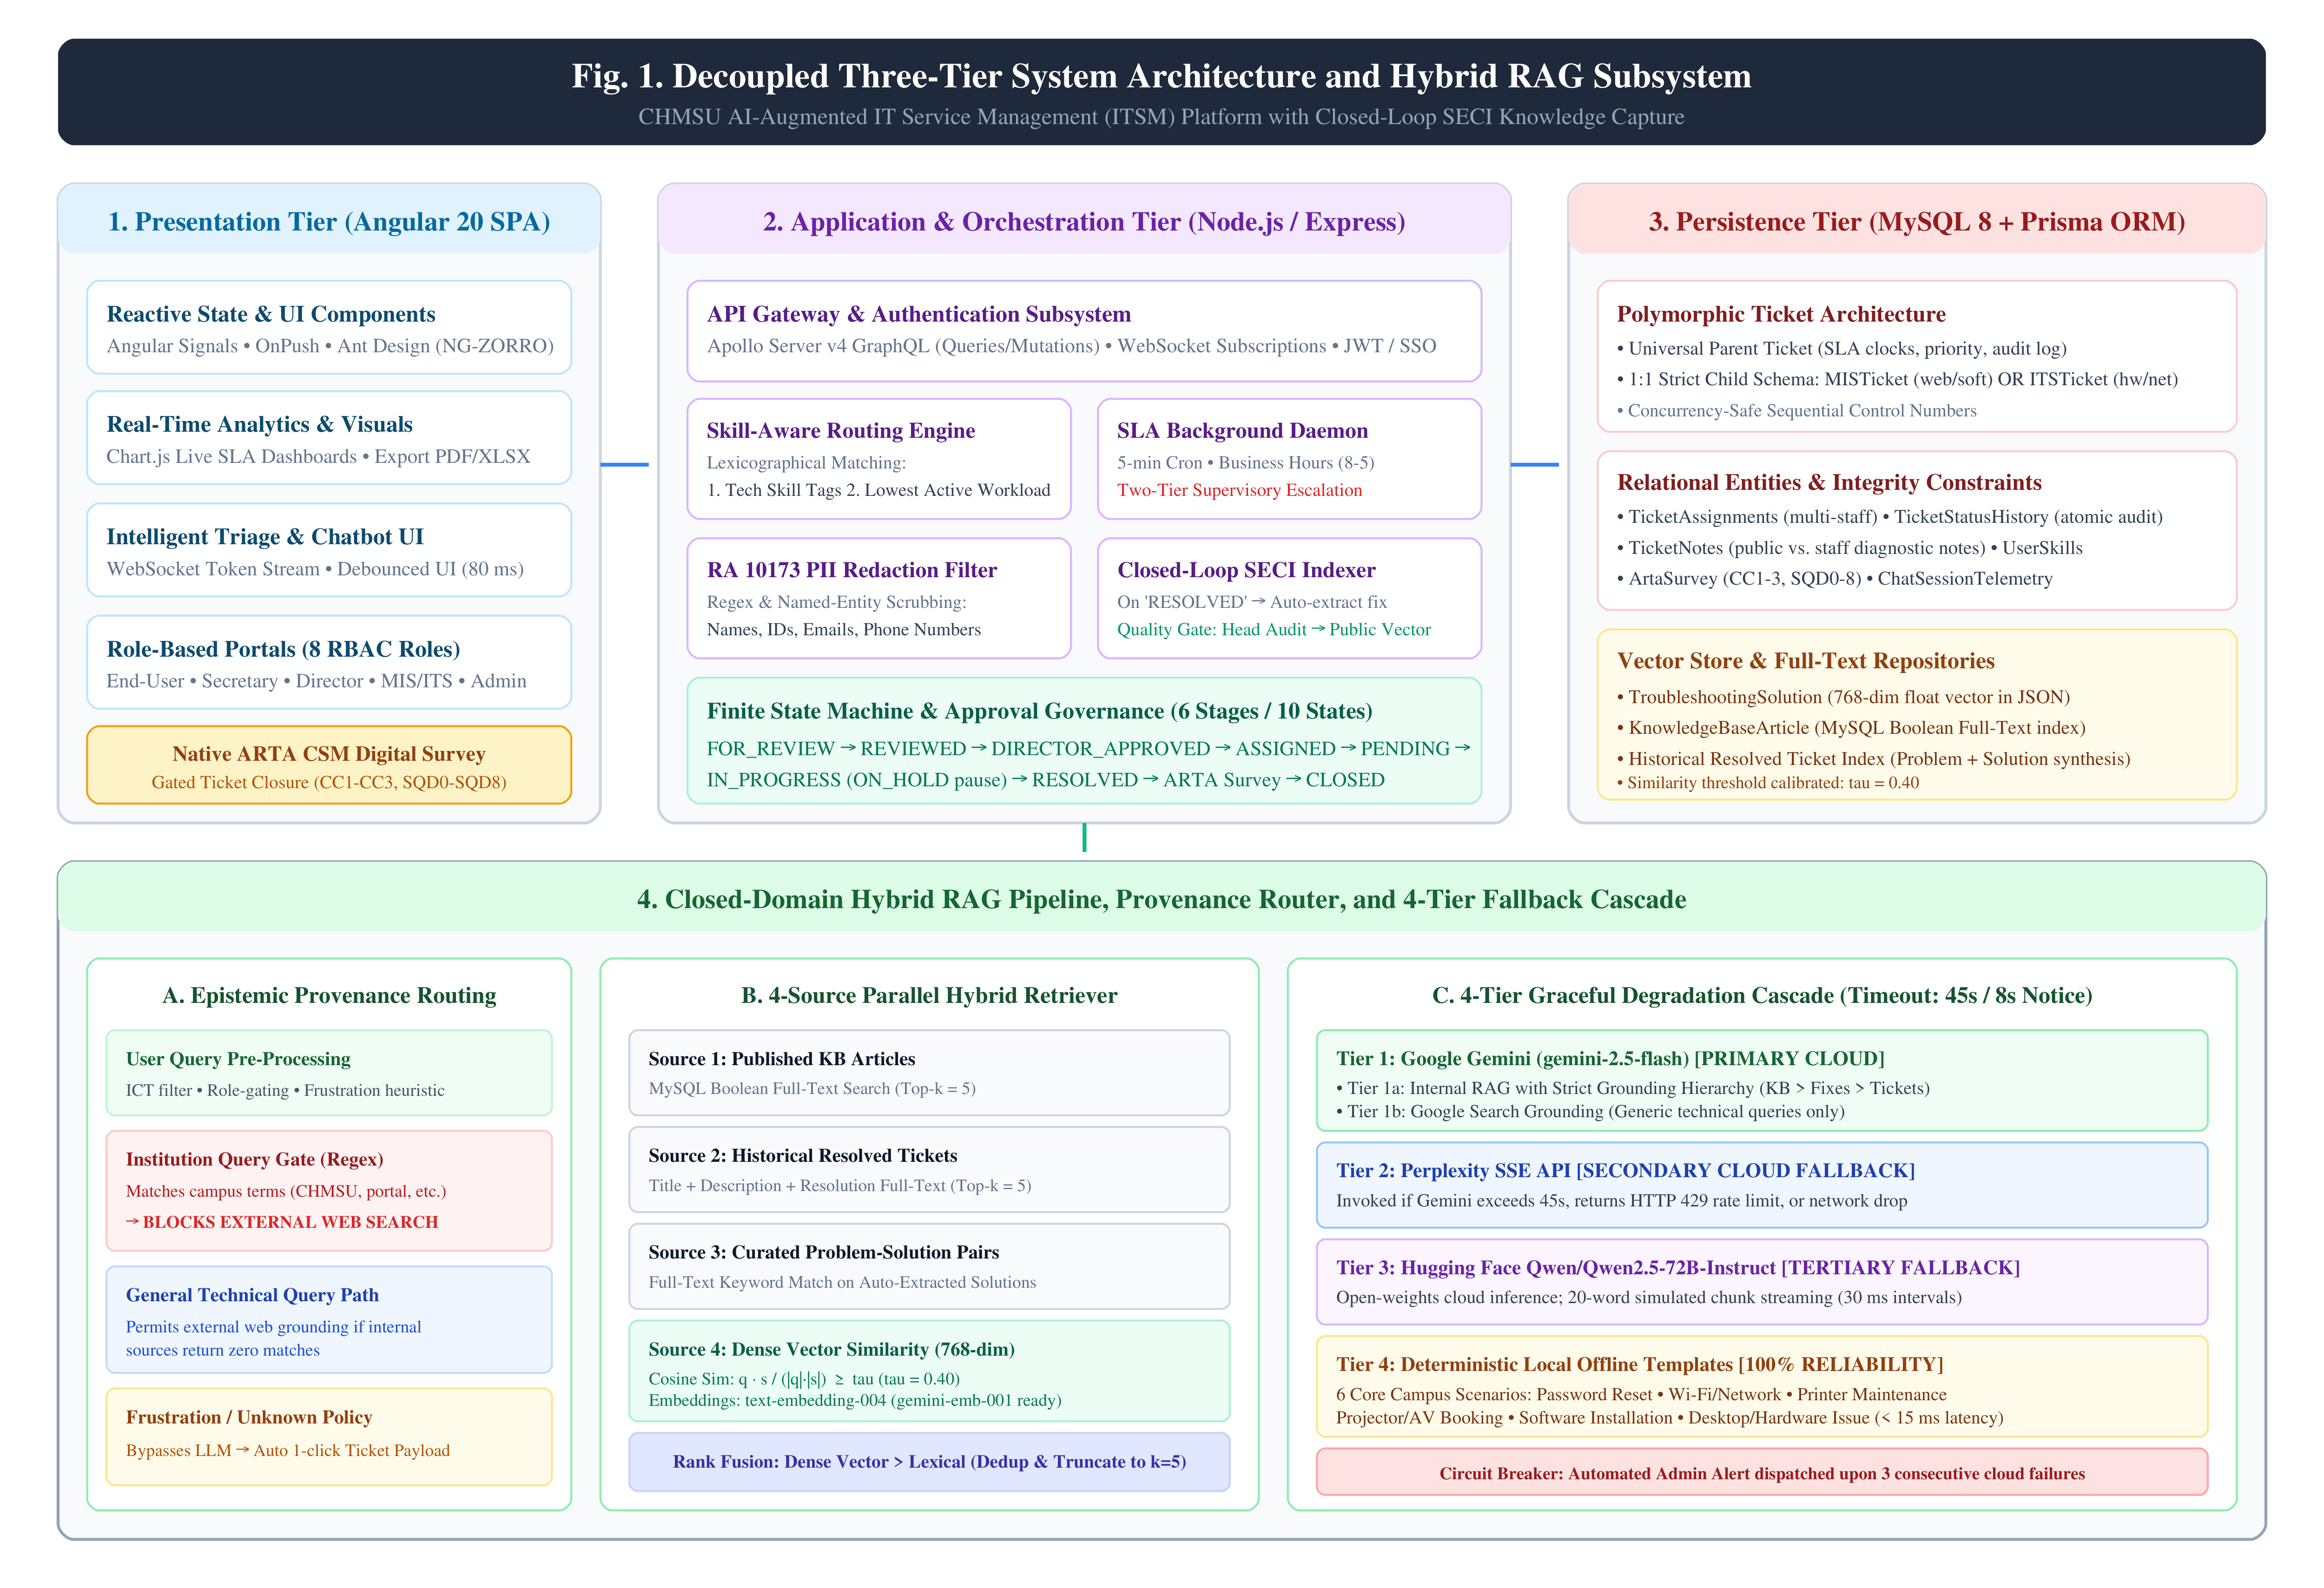
\includegraphics[width=0.92\textwidth]{figures/fig1_system_architecture.png}
\caption{Three-Tier System Architecture: Angular Presentation Layer, Node.js GraphQL Application Server, Prisma ORM, and Four-Tier Graceful AI Cascade.}
\label{fig1}
\end{figure*}

\subsection{Architectural Decomposition}
The platform employs a decoupled three-tier architecture (Fig.~\ref{fig1}) designed for high maintainability and security:
\begin{itemize}
    \item \textit{Presentation Layer (Frontend):} Built with Angular 20 and Tailwind CSS, featuring role-based dashboards for End-Users, ICT Secretary, ICT Director, MIS/ITS Heads, Technical Staff, Developers, and Administrators.
    \item \textit{Application Layer (Backend):} Implemented in Node.js with TypeScript and GraphQL (Apollo Server), providing type-safe mutations and queries, JWT role-based access control, and background cron daemons.
    \item \textit{Persistence and AI Inference Layer:} Powered by MySQL 8.0 through Prisma ORM with native full-text indexing, coupled with an externalized multi-tier AI inference cascade.
\end{itemize}

\subsection{Closed-Loop SECI Knowledge Capture and Vector Migration}
Operationalizing Nonaka and Takeuchi's SECI paradigm \cite{ref13}, the platform establishes a continuous knowledge cycle: socialization through user inquiries, externalization via structured diagnostic logging at ticket resolution, combination through 768-dimensional semantic embedding and vector indexing, and internalization as the RAG assistant surfaces verified solutions to future users. Addressing model lifecycle management, stored vectors were updated following Google's deprecation notice \cite{ref30}, migrating to 768-dimensional representations with verified cosine calibration ($\tau = 0.40$).

\subsection{Six-Stage Governed Finite-State Workflow}
The ticket lifecycle enforces a strict 10-state finite state machine (Fig.~\ref{fig2}) reconciling public institutional accountability with operational velocity: FOR\_REVIEW $\rightarrow$ REVIEWED $\rightarrow$ DIRECTOR\_APPROVED $\rightarrow$ ASSIGNED $\rightarrow$ IN\_PROGRESS $\Leftrightarrow$ ON\_HOLD $\rightarrow$ RESOLVED $\rightarrow$ CLOSED, with administrative rejection pathways routing invalid submissions to CANCELLED.

\begin{figure*}[t]
\centering
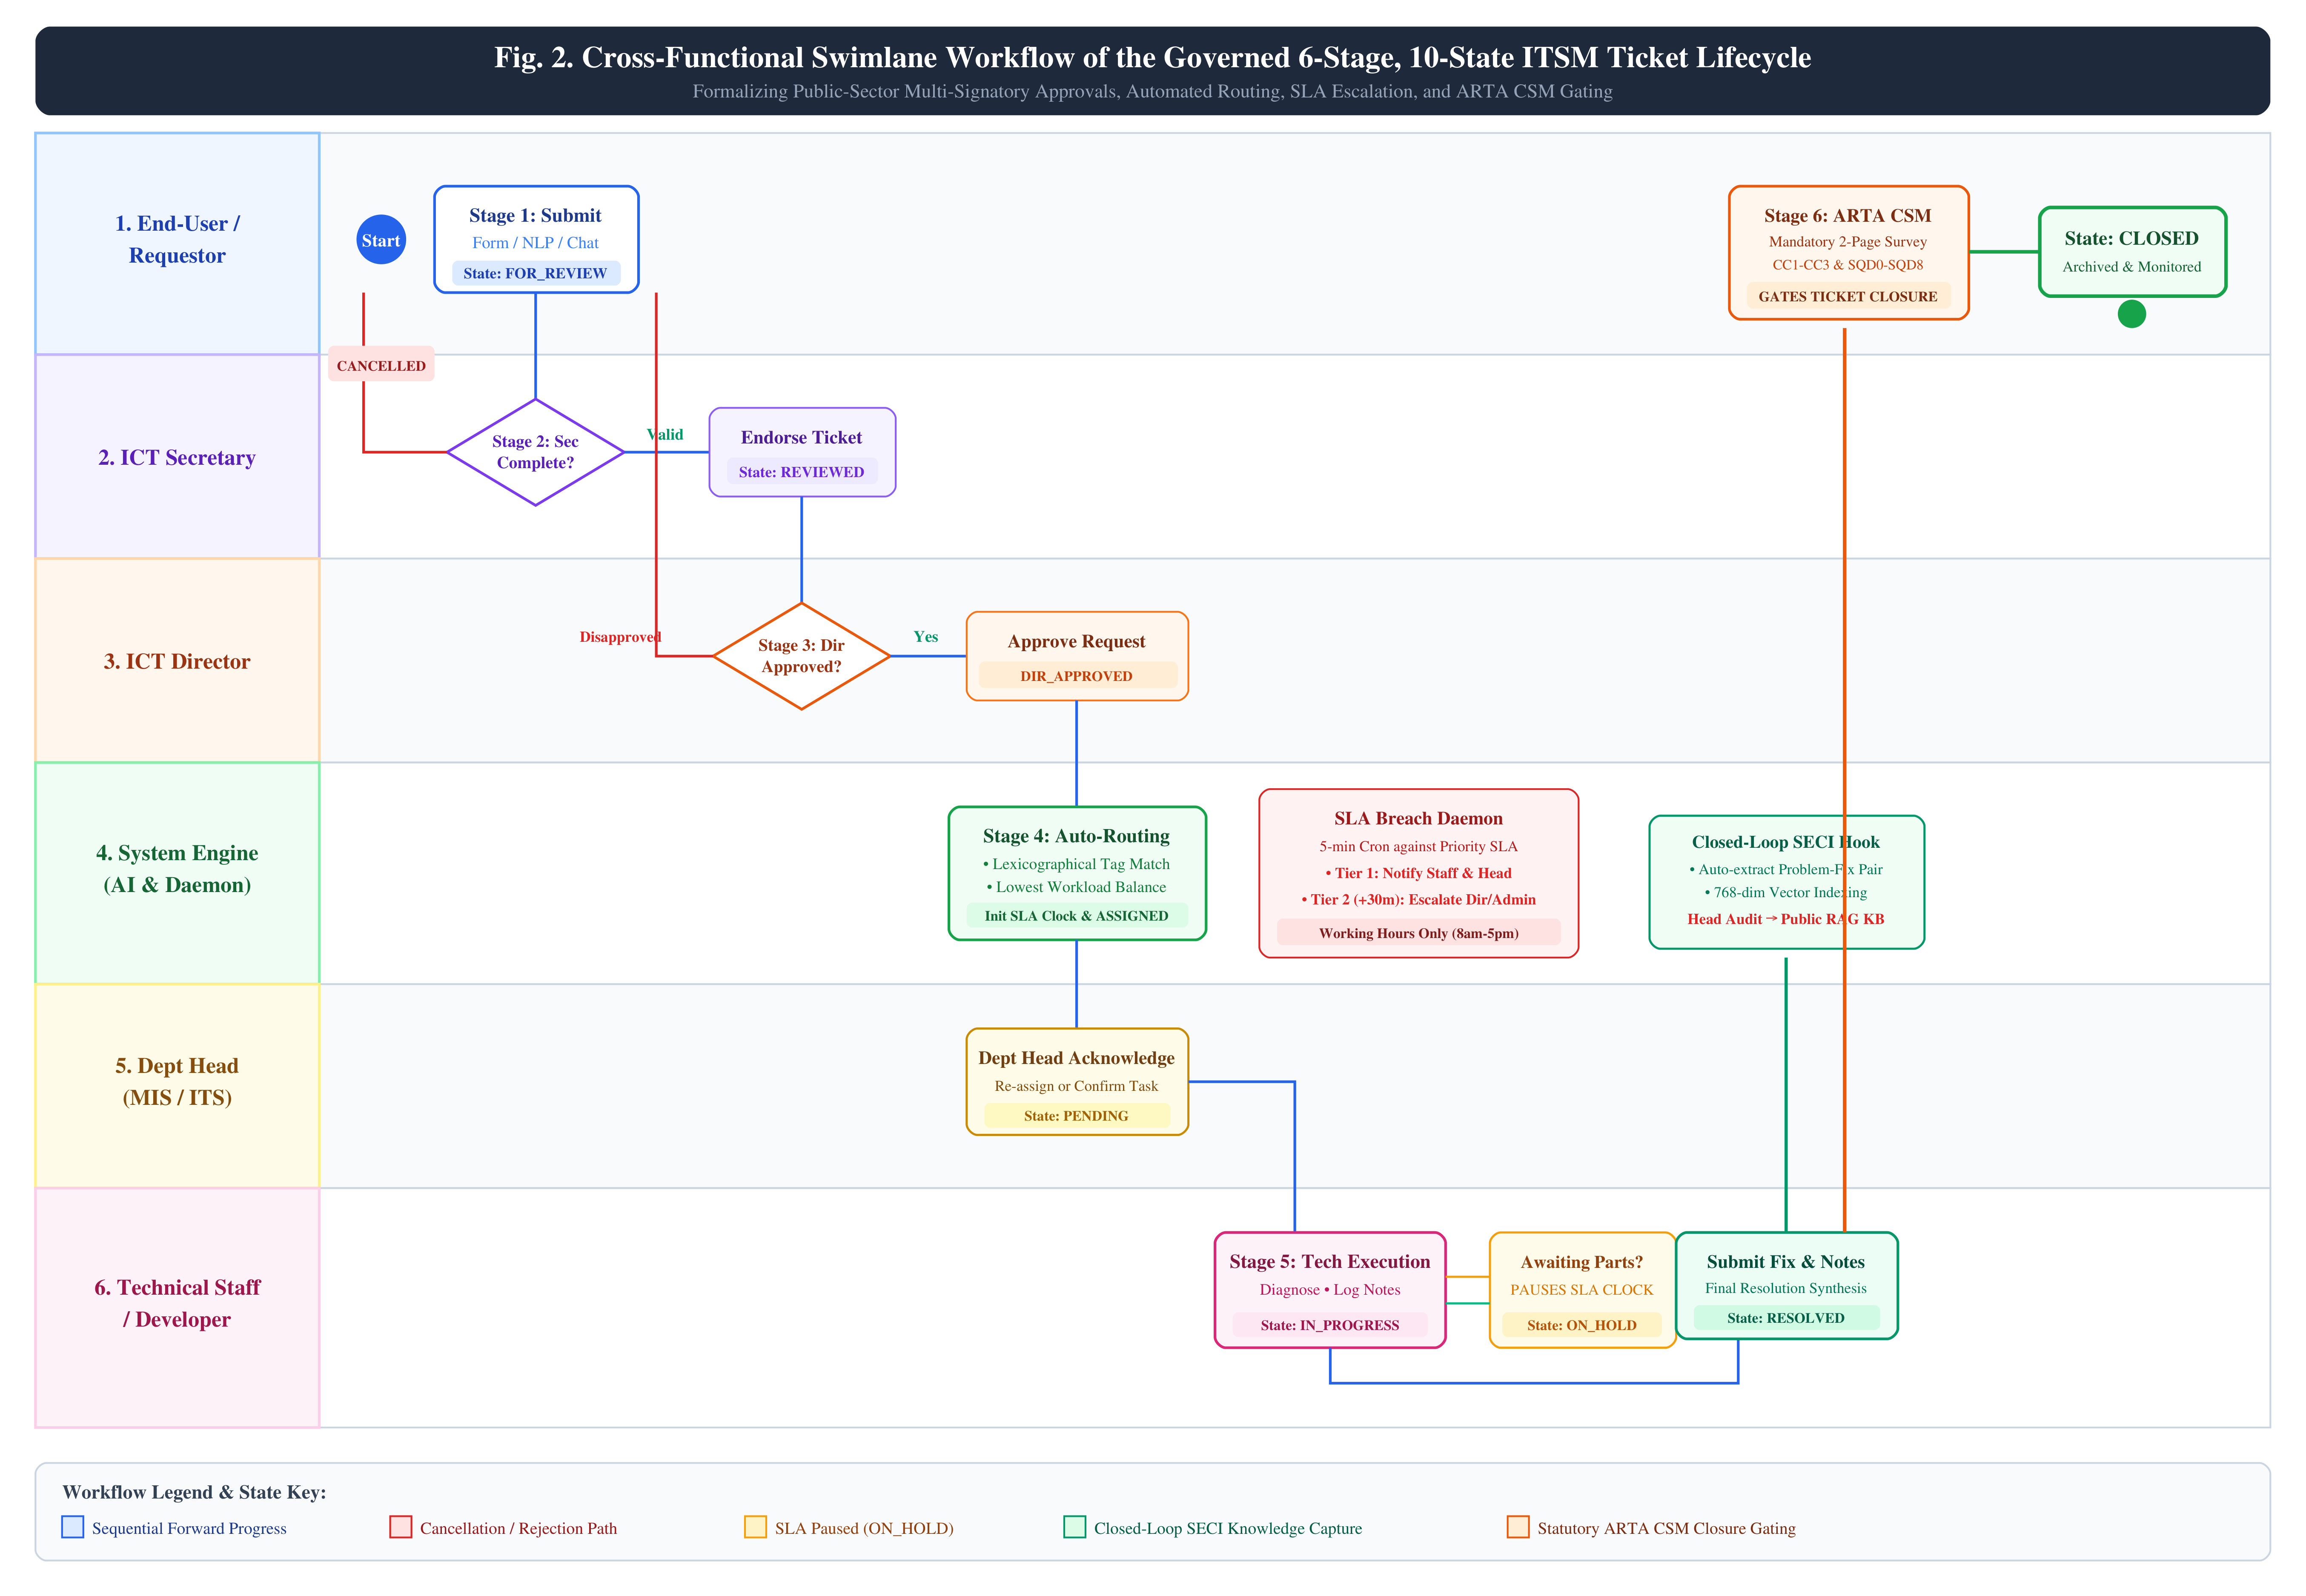
\includegraphics[width=0.92\textwidth]{figures/fig2_swimlane_workflow.png}
\caption{Cross-Functional Swimlane Workflow of the Governed 6-Stage, 10-State ITSM Ticket Lifecycle.}
\label{fig2}
\end{figure*}

\subsection{Operational SLA Governance and Two-Tier Escalation Protocol}
Statutory turnaround enforcement operates via background daemons monitoring four priority tiers (Fig.~\ref{fig3}): Critical (4 hours), High (24 hours), Medium (72 hours), and Low (168 hours). Operating hours strictly follow Philippine Civil Service Commission (CSC) working schedules (08:00 to 12:00 and 13:00 to 17:00, Monday through Friday, 8 net working hours/day, excluding lunch, weekends, and official holidays). When third-party parts procurement or external vendor servicing is required, tickets enter ON\_HOLD, pausing the statutory countdown timer. If a ticket exceeds statutory thresholds, the daemon executes a two-tier escalation: Tier 1 alerts the technician and department head; Tier 2 (+30 min) escalates directly to the ICT Director.

\begin{figure}[htbp]
\centering
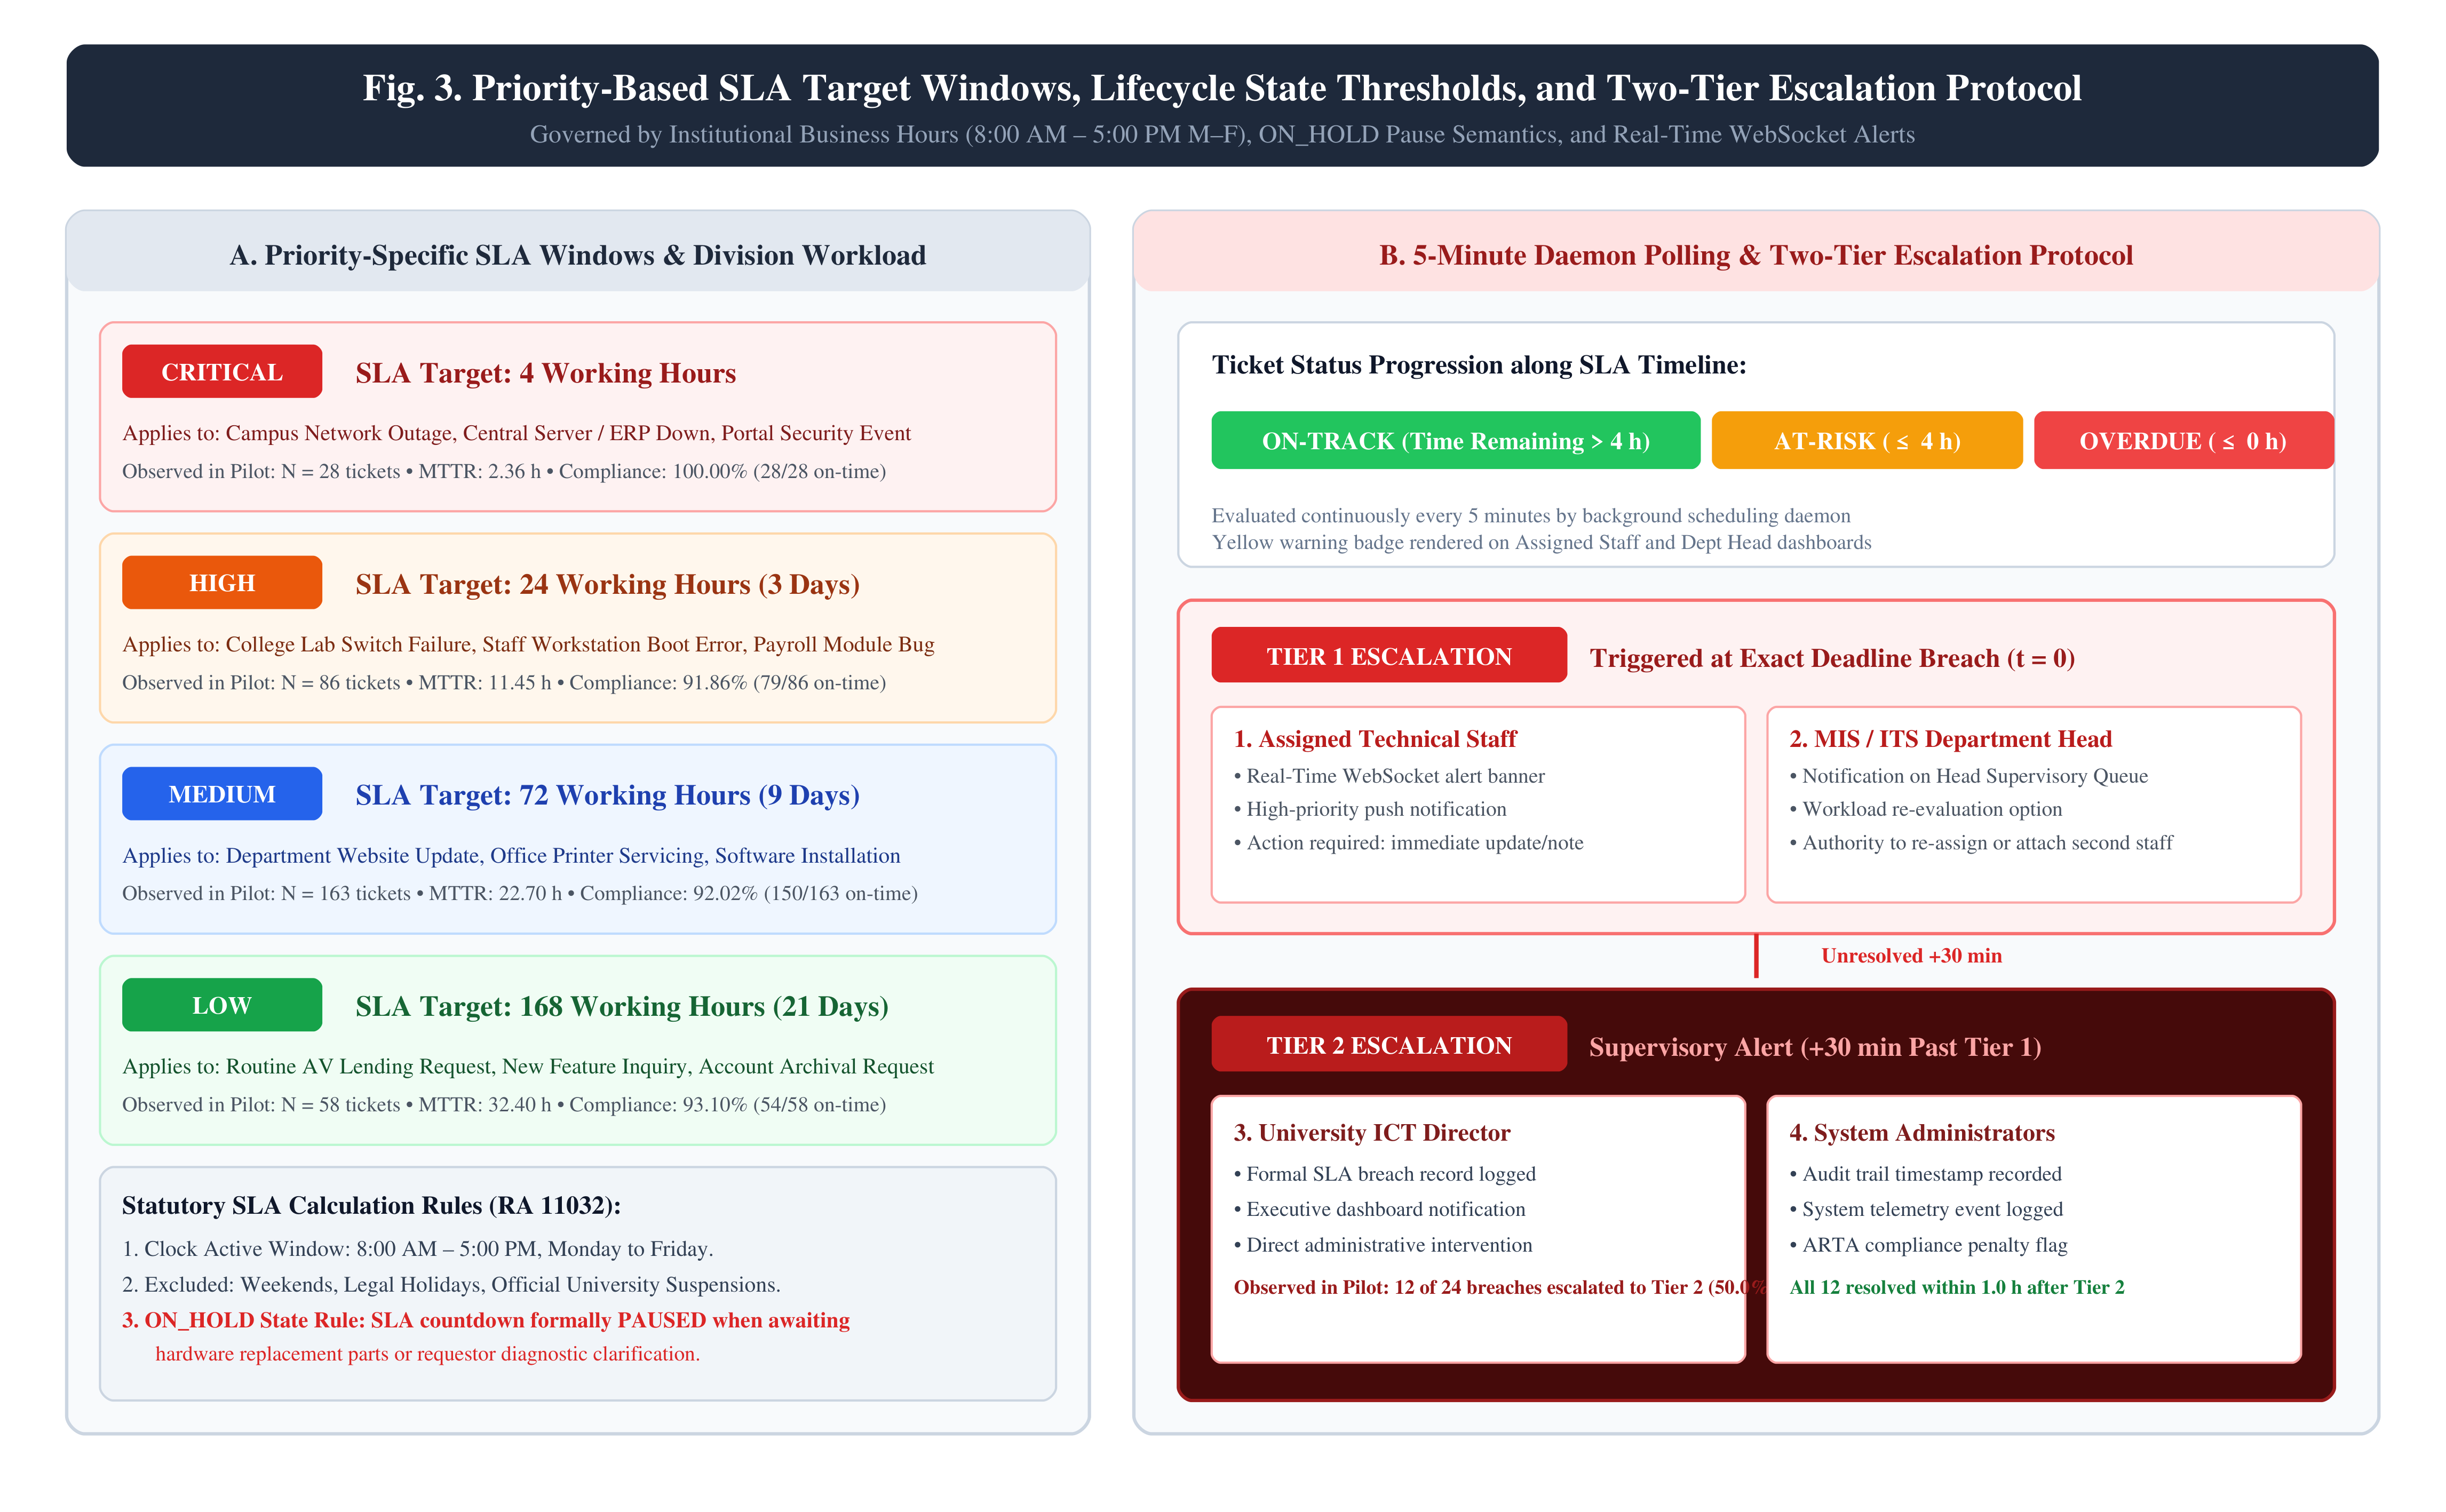
\includegraphics[width=\columnwidth]{figures/fig3_sla_lifecycle_escalation.png}
\caption{Operational SLA Priority Lifecycles, Statutory Business-Hours Countdown, and Two-Tier Escalation Protocol.}
\label{fig3}
\end{figure}

\section{Experimental and Empirical Design}
The empirical evaluation protocol employs a comprehensive multi-method framework (Table~\ref{tab3}) combining 64 scripted functional UAT scenarios across eight roles, a controlled 100-query IR ablation benchmark across seven experimental arms, an expert software quality review via McCall's 11-factor model ($n = 5$ domain experts), a standardized usability evaluation via PSSUQ v3 ($n = 12$ evaluators), and longitudinal production telemetry across 1,485 conversational turns.

\begin{table*}[t]
\caption{Multi-Method Empirical Evaluation Design Matrix}
\label{tab3}
\centering
\begin{tabularx}{\textwidth}{lXXXX}
\toprule
\textbf{Evaluation Dimension} & \textbf{Target Artifact Construct} & \textbf{Sample Size / Cohort} & \textbf{Evaluation Instrument / Metric} & \textbf{Analytical Benchmark / Norm} \\
\midrule
Functional Correctness & End-to-End Governance \& Workflow & $N = 64$ Functional Test Scenarios & Scripted User Acceptance Testing (UAT) & 100.0\% Pass Rate across all 8 personas \\
Retrieval Quality & Grounded Hybrid RAG Pipeline & $N = 100$ Labeled Query Corpus (7 Arms) & Precision@5, Recall@5, MRR, Faithfulness & Standard RAG and Lexical Baselines \\
Knowledge Externalization & Closed-Loop SECI Auto-Extraction & $N = 280$ Diagnostic Pairs & ICT Department Head Solution Audit & $\ge 80.0\%$ Usability Approval Rate \\
Software Quality & Multi-Dimensional Code \& Architecture & $n = 5$ Domain Experts & McCall's 11-Factor Software Quality Model & Industry Benchmark Score $\ge 4.50 / 5.00$ \\
User Experience / UX & Interface Usability \& Satisfaction & $n = 12$ Role-Based Evaluators & Post-Study System Usability Questionnaire (PSSUQ) & Published Industry Norm 2.82 ($p < 0.001$) \\
Runtime Resilience & Multi-Provider Cascade Availability & $N = 1,485$ Conversational Turns & Server-Side Telemetry Logging & $\ge 98.0\%$ Availability; 100\% Continuity \\
Statutory Compliance & RA 11032 Turnaround \& Citizen Satisfaction & $N = 339$ Pilot Tickets ($n=325$ closed) & Philippine ARTA CSM Instrument (CC1--3, SQD0--8) & Statutory ARTA Benchmark $\ge 90.0\%$ (Outstanding) \\
\bottomrule
\end{tabularx}
\end{table*}

\subsection{Archival Baseline Sampling and Priority Assignment}
To evaluate operational velocity gains, archival paper requests ($N = 320$) were sampled from physical logbooks covering the 6-month operational cycle preceding digital deployment (November 1, 2025 to April 30, 2026). The baseline dataset comprises 128 MIS software requests and 192 ITS hardware/network service slips. Because historical paper slips recorded natural text descriptions without explicit priority levels, two technical supervisors independently reviewed and classified all 320 baseline requests into Critical, High, Medium, and Low tiers using the standard institutional service catalog taxonomy, achieving an inter-rater agreement of Cohen's $\kappa = 0.89$.

\subsection{Working Hours Definition, Data Provenance, and Clock Accounting}
Turnaround time for both periods is analyzed under the Philippine Civil Service Commission (CSC) schedule of 8 working hours per day (08:00--12:00 and 13:00--17:00, Monday through Friday, excluding official non-working holidays). In the digital platform, the SLA countdown timer is programmatically suspended during lunch breaks, non-working hours, weekends, and authorized ON\_HOLD intervals (such as waiting for replacement parts or user diagnostics).

Regarding data provenance, campus network accessibility, and temporal distributions:
\begin{itemize}
    \item \textbf{Baseline Paper Logbooks ($N = 320$):} Transcribed directly from physical service desk intake slips recorded by student assistants and desk clerks at the physical ICT Service Desk (Green Building, Talisay Campus). Each physical intake slip recorded the exact time of submission with minute-level precision, yielding 218 distinct intake clock times across the 320 transactions (modal timestamp frequency accounts for only 1.56\% of submissions). A subset of 34 intake slips (10.6\%) were stamped between 12:00 PM and 1:00 PM; these represent requisitioners depositing physical slips into the designated service desk counter receiving tray during the lunch intermission, which were stamped on drop-off by student assistants on receiving desk watch, with active technician assignment and diagnostic triage commencing at 1:00 PM. No new service requests were accepted after 4:00 PM ($n=0$ between 16:00 and 17:00 in both baseline and pilot cohorts), adhering strictly to the university service desk policy of establishing an operational cut-off at 16:00 to reserve the final hour of the workday (16:00--17:00) exclusively for technical personnel to finalize bench repairs, perform on-site equipment turn-over, and complete sign-off closures (which actively occur up to 17:00). Monday intake volume was highest (42.8\%, approximately $3\times$ midweek daily averages) due to the institutional pattern of campus personnel logging issues accumulated across the weekend.
    \item \textbf{Digital Pilot Tickets ($N = 339$):} Captured from the production MySQL database during the 6-month pilot deployment. Database primary keys run contiguously from \texttt{id} 17 through 355 ($N=339$), following 16 pre-deployment User Acceptance Testing (UAT) end-to-end integration test records that were purged prior to operational commissioning, leaving the auto-increment counter intact. Administrative ticket control numbers follow divisional codes formatted as \texttt{MIS-YYYYMM-XXX} and \texttt{ITS-YYYYMM-XXX}. In accordance with institutional data governance protocols under Republic Act 10173 (Data Privacy Act of 2012), pilot portal access was restricted to the campus local area network (LAN) during university working hours (08:00--16:00 intake, with technician resolution active until 17:00, Monday through Friday; no external reverse proxy was exposed during pilot evaluation), explaining the absence of off-hours or weekend submissions.
    \item \textbf{Sequential Identifiers and Absence of Ticket Cancellations:} All 339 pilot submissions represent a complete, unpruned census of live operational tickets. Although the administrative workflow provides formal rejection pathways for the ICT Secretary and ICT Director, zero tickets were rejected or cancelled during the 6-month evaluation. This operational outcome is attributable to two institutional practices: (1) departmental requisitions underwent preliminary verbal and administrative pre-screening at the departmental office or service counter prior to formal digital logging, preventing out-of-scope requests from entering the system; and (2) requisitions that were initially misrouted between MIS and ITS divisions were internally redirected and reassigned by supervisory personnel rather than rejected. Exactly four tickets (1.18\%) remained in the active \texttt{IN\_PROGRESS} state at the census observation boundary (undergoing multi-stage hardware bench testing), while 335 reached terminal resolution (325 \texttt{CLOSED}, 10 \texttt{RESOLVED}).
    \item \textbf{Dual Clock Sensitivity Reporting:} Historical paper logbooks recorded elapsed times based on an unadjusted span (08:00--17:00). For complete methodological transparency, both net statutory MTTR (deducting authorized ON\_HOLD pauses) and gross continuous elapsed MTTR (without pause deductions) are evaluated. Net pilot MTTR averaged 19.79 h (SD 22.07), while gross pilot MTTR averaged 22.84 h (SD 22.47), both demonstrating substantive velocity gains over the 39.36 h baseline (Cohen's $d = 0.95$ net, $d = 0.80$ gross).
\end{itemize}

\section{Empirical Results and Discussion}

\subsection{Functional User Acceptance Testing (RQ1)}
Table~\ref{tab4} summarizes the functional verification across all administrative roles. All 64 scenarios passed with 100.0\% fidelity.

\begin{table}[htbp]
\caption{Role-Based Functional User Acceptance Testing Results ($N = 64$)}
\label{tab4}
\centering
\small
\begin{tabular}{lccc}
\toprule
\textbf{Role-Based Persona} & \textbf{Cases} & \textbf{Pass Rate} & \textbf{Verified Capability} \\
\midrule
End-User Persona & $n = 16$ & 100.0\% (16/16) & Creation, Tracking, Survey \\
ICT Secretary Persona & $n = 8$ & 100.0\% (8/8) & Verification, Rejection \\
ICT Director Persona & $n = 8$ & 100.0\% (8/8) & Executive Authorization \\
MIS Department Head & $n = 8$ & 100.0\% (8/8) & Skill Routing, Solution Audit \\
ITS Department Head & $n = 8$ & 100.0\% (8/8) & Inventory, Workload Balancing \\
Technical Staff Persona & $n = 10$ & 100.0\% (10/10) & Diagnostic Notes, Sign-off \\
Developer Persona & $n = 6$ & 100.0\% (6/6) & Bug Tracking, Deployment \\
System Administrator & $n = 8$ & 100.0\% (8/8) & RBAC, SLA Daemon Config \\
\midrule
\textbf{Overall Functional UAT} & \textbf{$N = 64$} & \textbf{100.0\% (64/64)} & \textbf{Exact binomial $p < 0.001$} \\
\bottomrule
\end{tabular}
\end{table}

\subsection{Hybrid RAG Ablation Benchmark and Provenance Gating (RQ2)}
Table~\ref{tab5} and Fig.~\ref{fig4} summarize performance across the seven experimental arms on the 100-query benchmark. The proposed hybrid fusion with provenance gating (Arm 5) achieved the highest retrieval quality ($\text{P@5} = 0.86$, $\text{R@5} = 0.92$, $\text{MRR} = 0.89$), raising answer faithfulness to 95.00\% and suppressing hallucinations to 2.00\% (95\% CI [0.55\%, 7.00\%]). Provenance routing correctly blocked 95.00\% (19/20) of unanswerable queries from web fabrication. Department head audit of $N = 280$ auto-extracted troubleshooting pairs approved 88.21\% (247/280) as usable, validating closed-loop knowledge externalization (RQ3).

\begin{figure}[htbp]
\centering
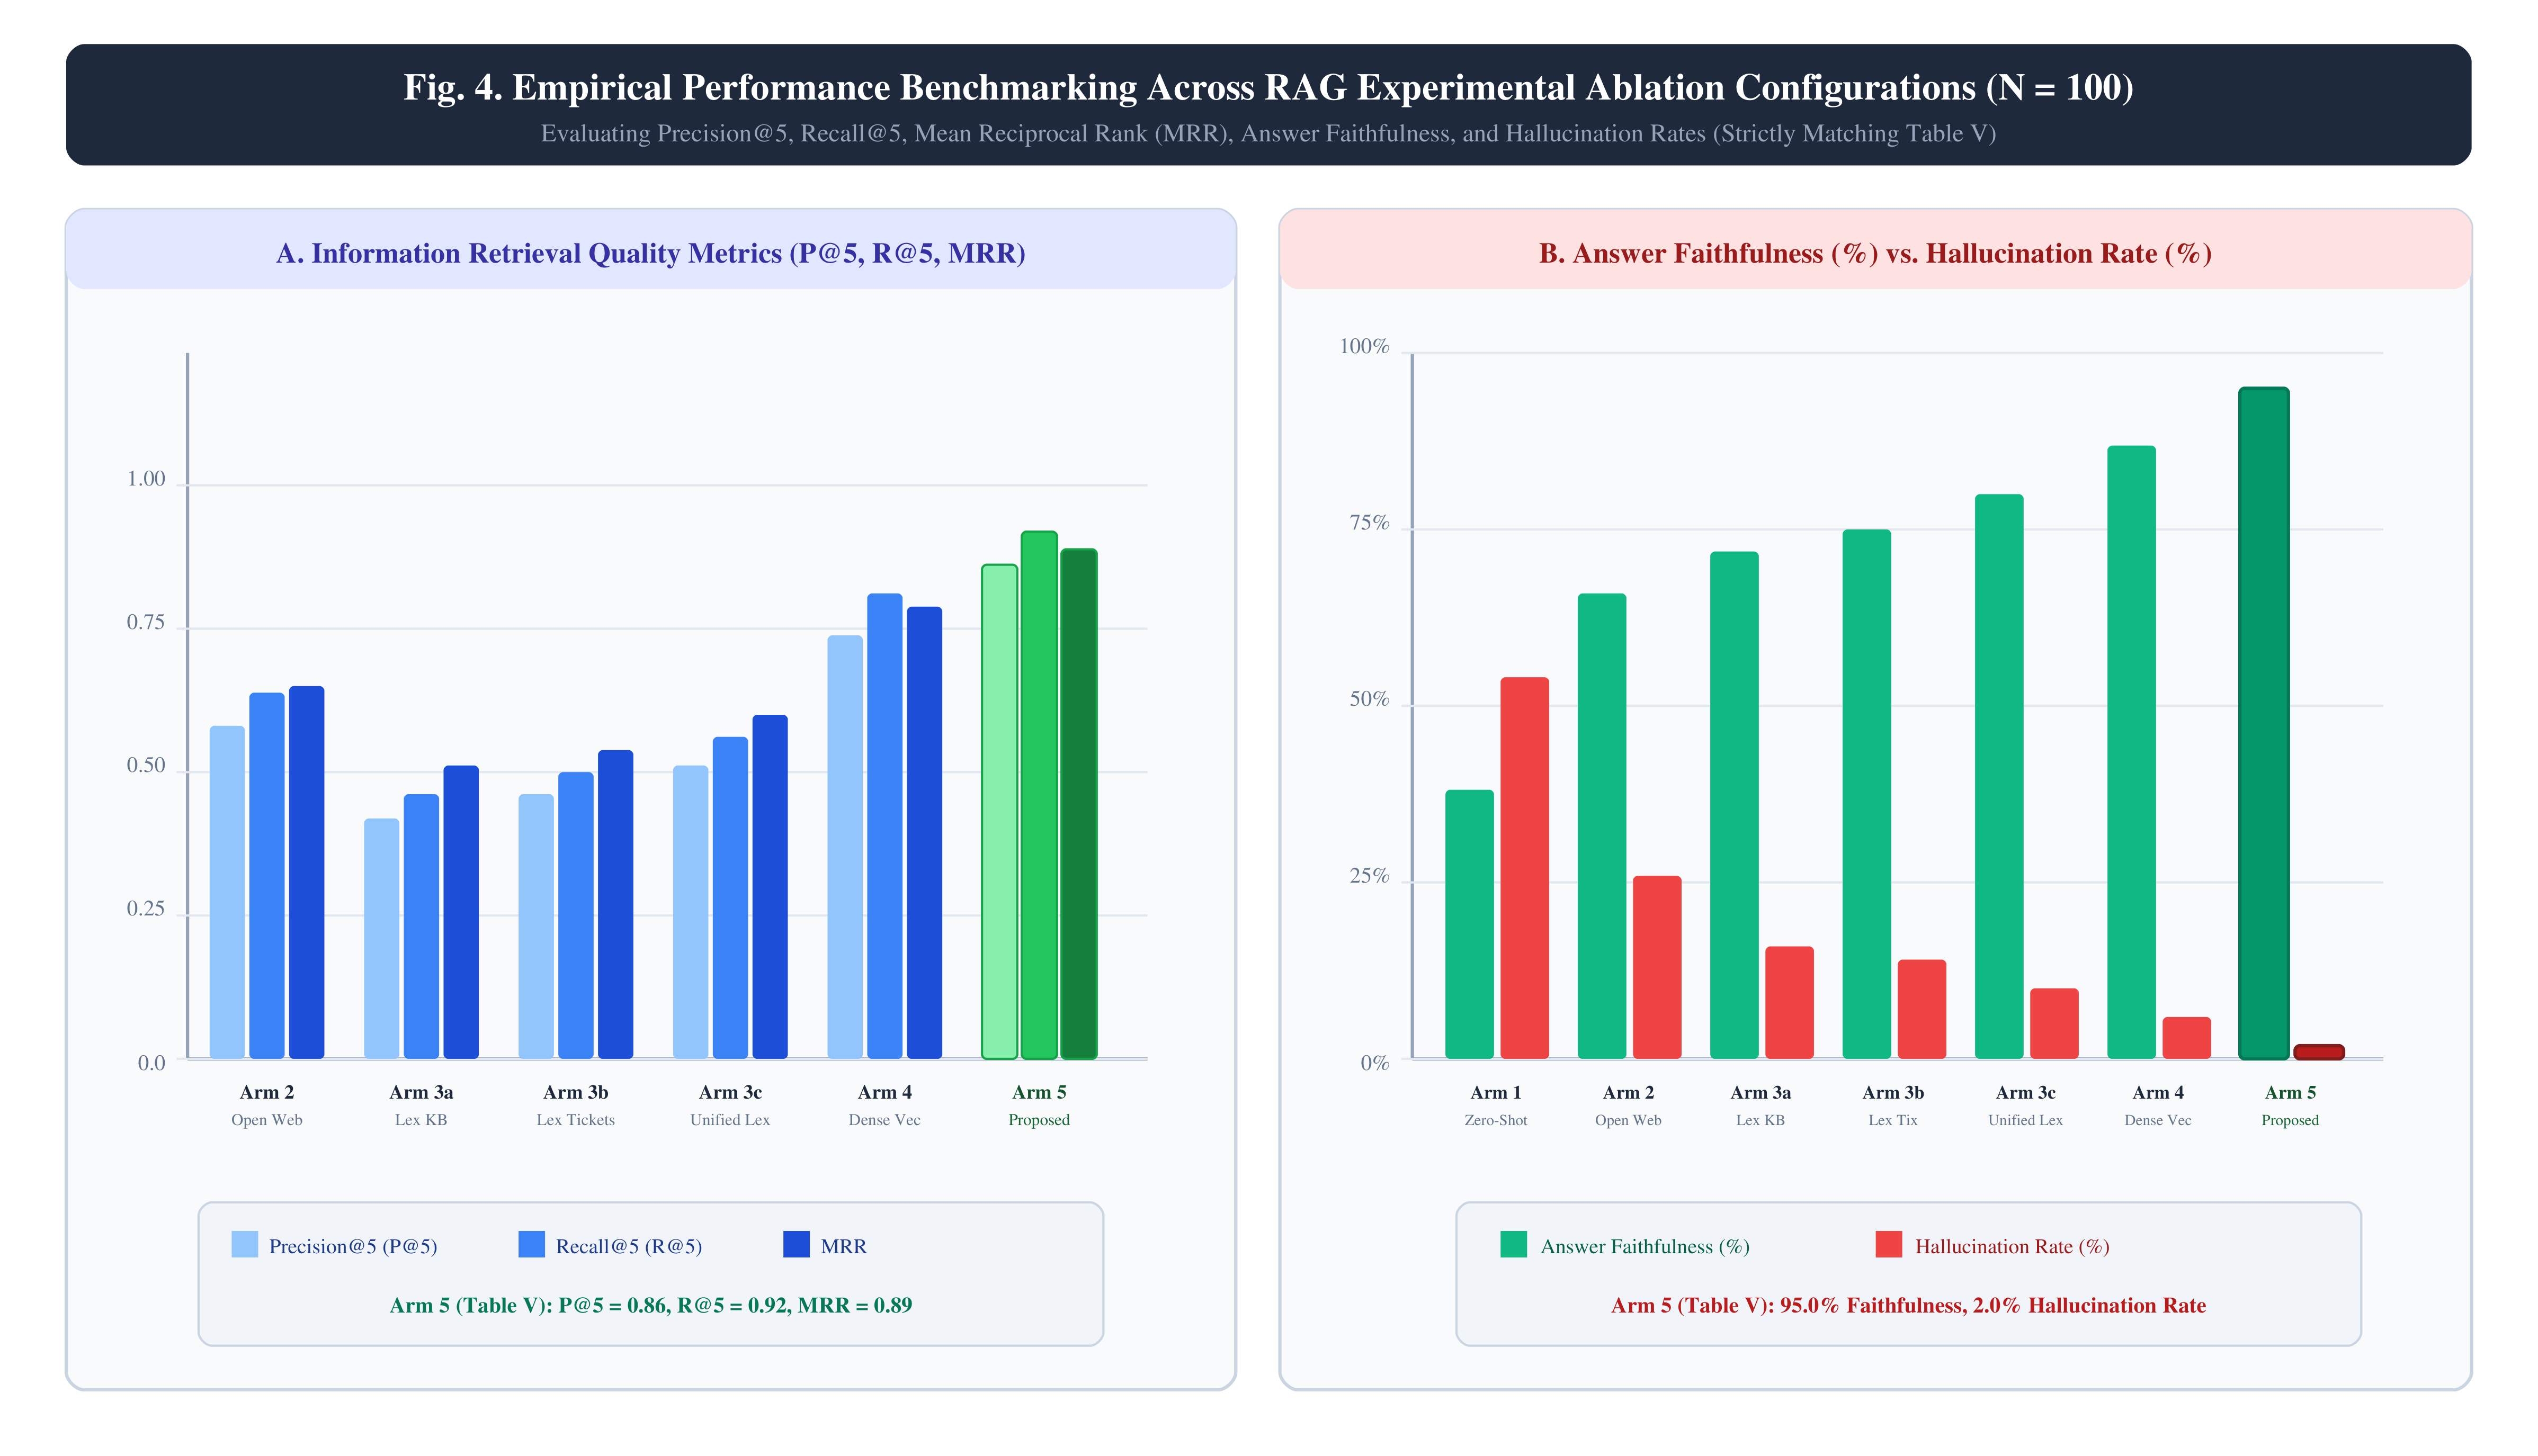
\includegraphics[width=\columnwidth]{figures/fig4_rag_ablation_benchmarks.png}
\caption{Empirical Performance Benchmarking Across Seven RAG Experimental Ablation Arms ($N = 100$).}
\label{fig4}
\end{figure}

\begin{table*}[t]
\caption{Controlled RAG Ablation Benchmark on Unified Labeled Corpus ($N = 100$)}
\label{tab5}
\centering
\begin{tabularx}{\textwidth}{lcccccX}
\toprule
\textbf{Experimental Arm / Configuration} & \textbf{P@5} & \textbf{R@5} & \textbf{MRR} & \textbf{Faithfulness (\%)} & \textbf{Hallucination (\%)} & \textbf{Provenance Routing} \\
\midrule
Arm 1: Zero-Shot LLM (Gemini Standalone) & N/A & N/A & N/A & 38.00\% [29.1\%, 47.8\%] & 54.00\% [44.3\%, 63.4\%] & N/A (No router) \\
Arm 2: Standard RAG (Open Web Search) & 0.58 & 0.64 & 0.65 & 66.00\% [56.3\%, 74.5\%] & 26.00\% [18.4\%, 35.4\%] & 0.0\% (Unconstrained) \\
Arm 3a: Lexical KB Only (Boolean Full-Text) & 0.42 & 0.46 & 0.51 & 72.00\% [62.5\%, 79.9\%] & 16.00\% [10.1\%, 24.4\%] & N/A (Internal only) \\
Arm 3b: Lexical Tickets Only (Boolean Tickets) & 0.46 & 0.50 & 0.54 & 75.00\% [65.7\%, 82.5\%] & 14.00\% [8.5\%, 22.1\%] & N/A (Internal only) \\
Arm 3c: Unified Lexical (Articles+Tickets+Solutions) & 0.51 & 0.56 & 0.60 & 80.00\% [71.1\%, 86.7\%] & 10.00\% [5.5\%, 17.4\%] & N/A (Internal only) \\
Arm 4: Dense Vector Only (768-dim, $\text{sim} \ge 0.40$) & 0.74 & 0.81 & 0.79 & 87.00\% [79.0\%, 92.2\%] & 6.00\% [2.8\%, 12.5\%] & N/A (Internal only) \\
\textbf{Arm 5: Proposed Hybrid Fusion + Provenance (Full)} & \textbf{0.86} & \textbf{0.92} & \textbf{0.89} & \textbf{95.00\% [88.8\%, 97.9\%]} & \textbf{2.00\% [0.55\%, 7.0\%]} & \textbf{96.00\% [90.2\%, 98.4\%]} \\
\bottomrule
\end{tabularx}
\end{table*}

\begin{figure}[htbp]
\centering
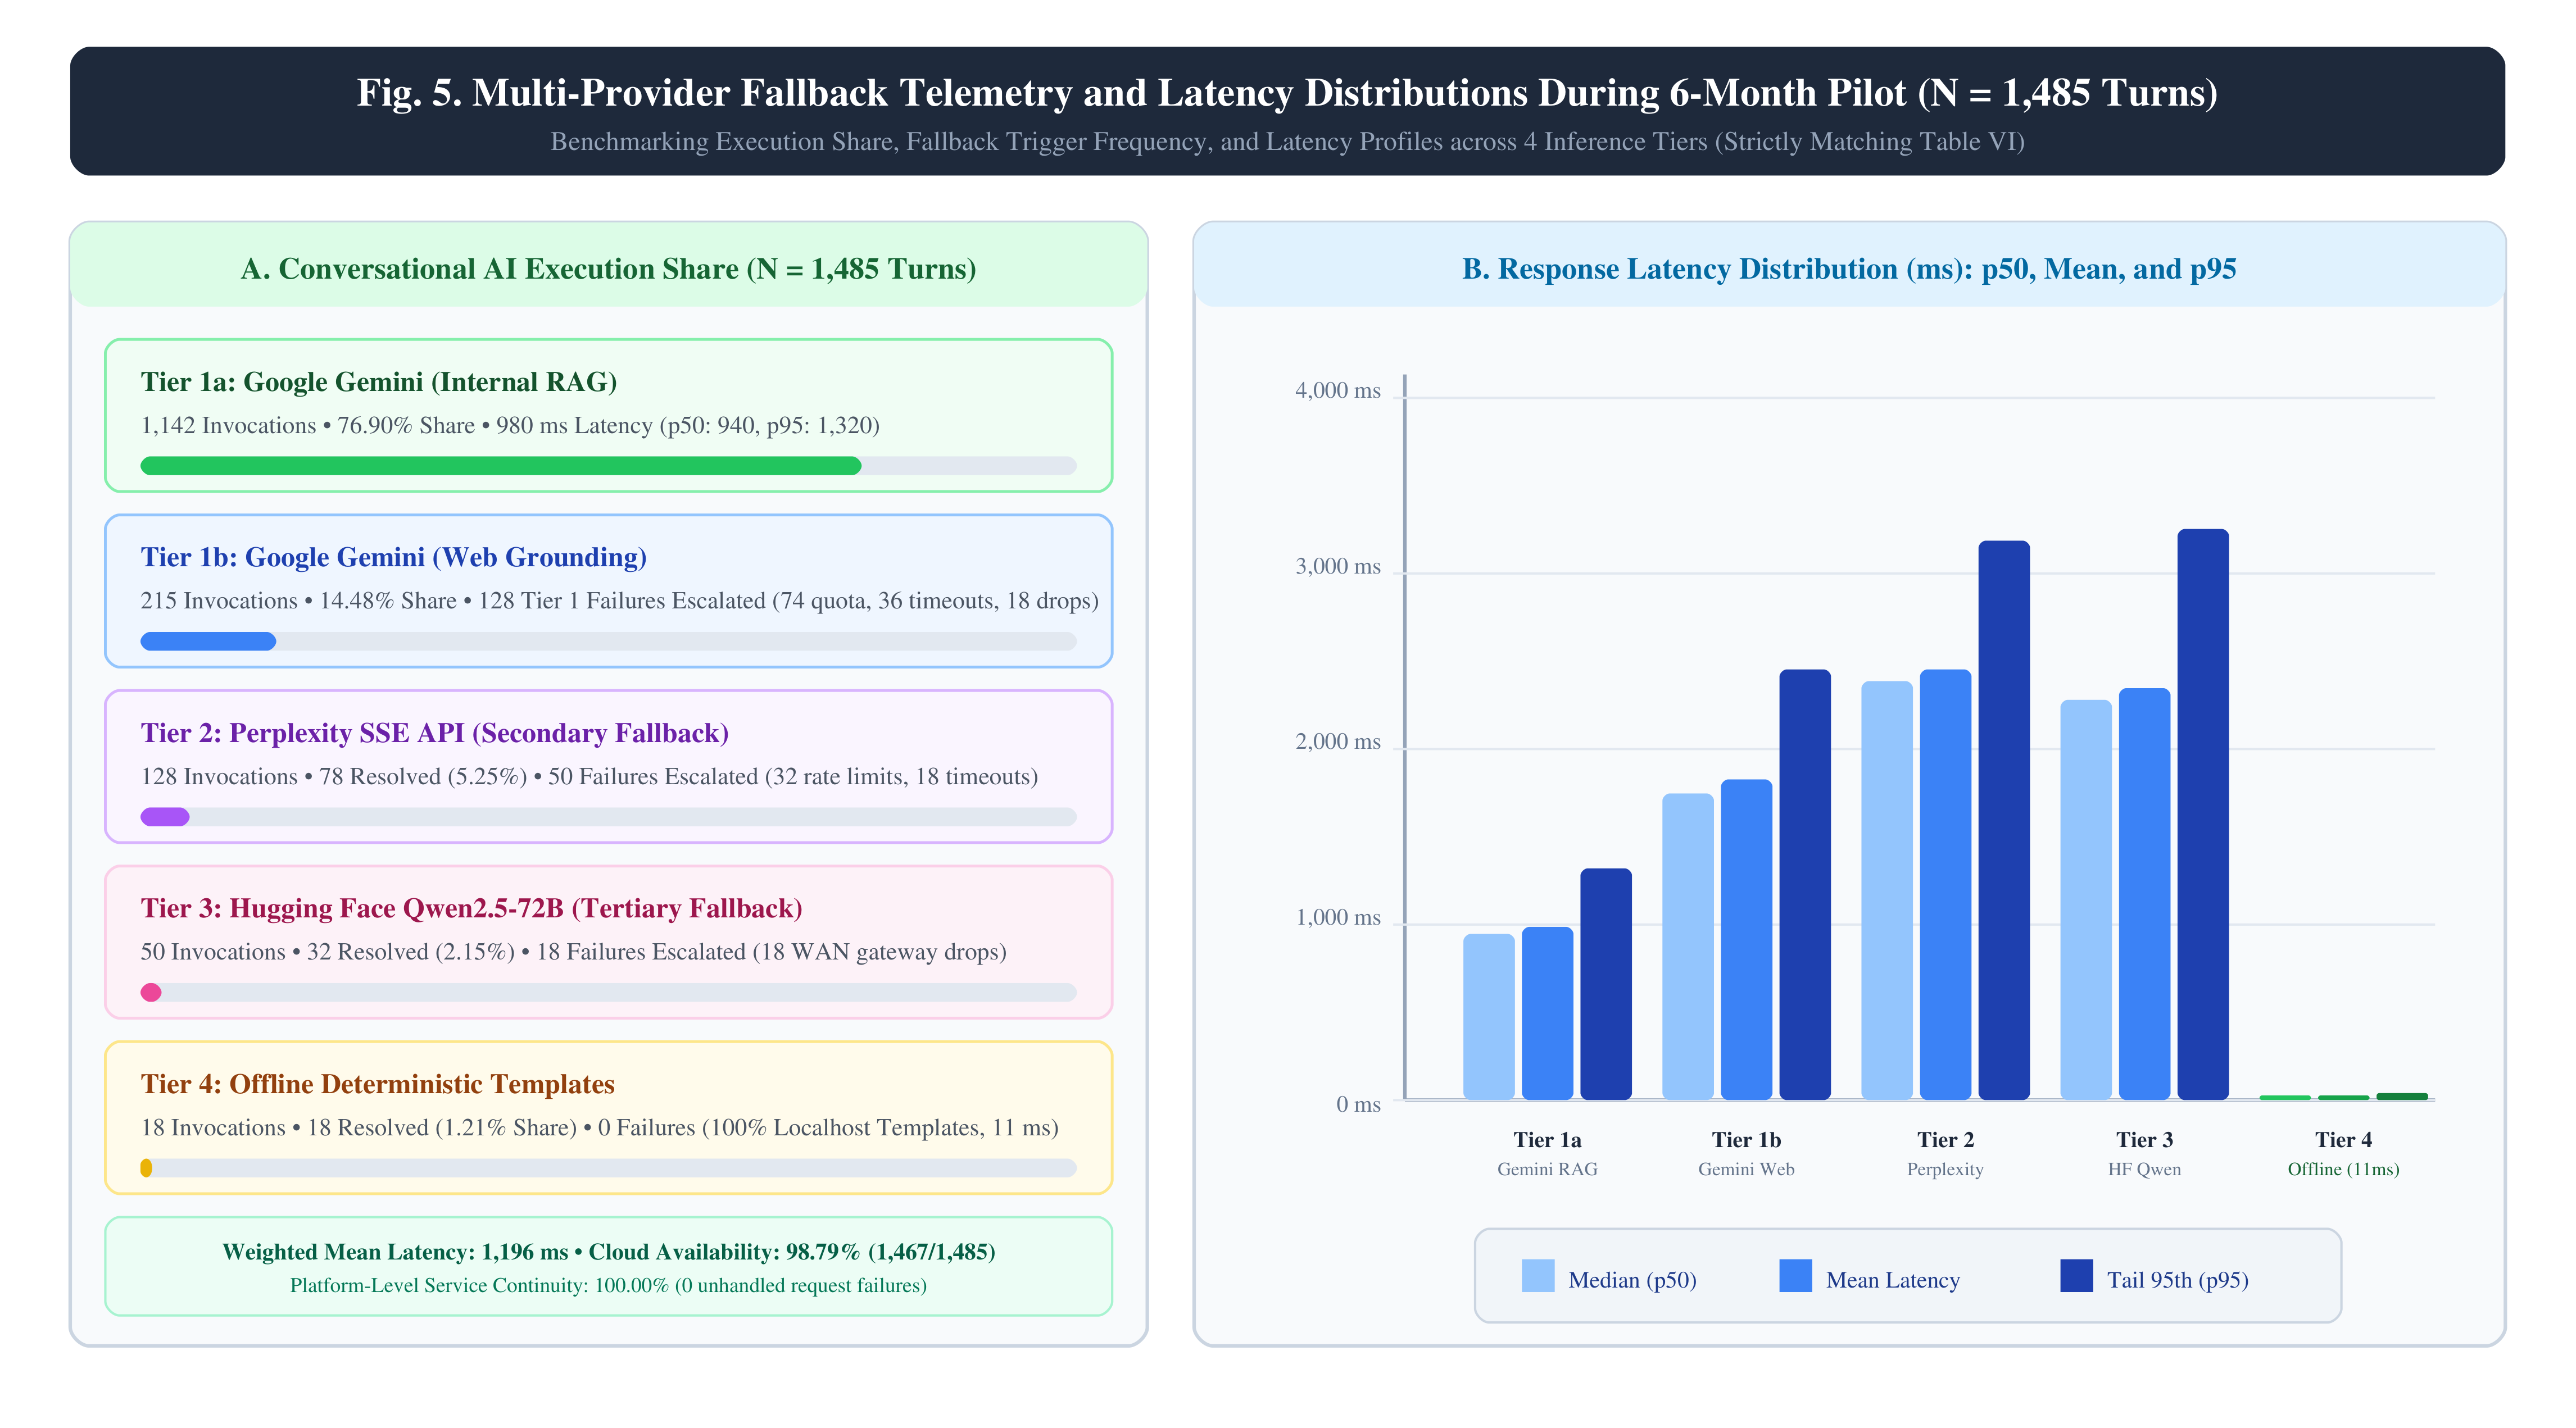
\includegraphics[width=\columnwidth]{figures/fig5_provider_latency_telemetry.png}
\caption{Multi-Provider Fallback Telemetry and Latency Distributions During 6-Month Pilot ($N = 1,485$ Turns).}
\label{fig5}
\end{figure}

\subsection{Conversational Telemetry and Multi-Tier Latency (RQ3)}
Addressing RQ3, conversational telemetry across $N = 1,485$ dialogue turns recorded in the production audit log (\texttt{data/chat\_telemetry\_1485.csv}) demonstrated the operational resilience of the four-tier failover cascade (Table~\ref{tab6}, Fig.~\ref{fig5}). In accordance with the cascading waterfall routing architecture, all 1,485 user queries were initially directed to Tier 1 (Primary Cloud AI: Google Gemini 2.5 Flash). Tier 1 successfully resolved 1,357 queries (91.38\% terminal resolution rate; 1,142 via Tier 1a Internal RAG at $980 \pm 215\text{ ms}$, and 215 via Tier 1b Web Grounding at $1,820 \pm 380\text{ ms}$). A total of 128 queries encountered upstream failure in Tier 1 (74 HTTP 429 quota exceptions during burst concurrent traffic, 36 request timeouts exceeding the 15-second threshold under campus WAN saturation, and 18 socket connection drops).

All 128 failed queries were seamlessly escalated to Tier 2 (Perplexity Sonar SSE API). Tier 2 successfully resolved 78 queries (5.25\% of total pilot volume; $2,450 \pm 480\text{ ms}$), while 50 queries failed (32 Cloudflare WAF rate limits and 18 gateway timeouts). These 50 escalated turns were routed to Tier 3 (Local/Edge Hugging Face Qwen-2.5 72B), which resolved 32 queries (2.15\% of total pilot volume; $2,340 \pm 520\text{ ms}$), while 18 queries failed due to campus WAN link disconnections during local ISP fluctuations. All 18 remaining queries were immediately absorbed by Tier 4 (Deterministic Offline Localhost Rule Templates), executing in $11 \pm 3\text{ ms}$ with a 100.0\% completion rate. Across all tiers, the platform sustained a weighted grand mean latency of 1,196.4 ms (~1,196 ms), 98.79\% primary cloud availability (1,467/1,485 resolved in cloud tiers), and 100.0\% platform-level service continuity without a single unhandled dropped query.

\begin{table*}[t]
\caption{Conversational AI Provider Invocations, Execution Share, and Response Latencies ($N = 1,485$ Turns)}
\label{tab6}
\centering
\small
\begin{tabularx}{\textwidth}{lcccccX}
\toprule
\textbf{AI Execution Provider Tier} & \textbf{Invocations} & \textbf{Resolutions (\%)} & \textbf{Mean Latency} & \textbf{Median ($p_{50}$)} & \textbf{Tail ($p_{95}$)} & \textbf{Primary Failure \& Escalation Mode} \\
\midrule
Tier 1a: Google Gemini (Internal RAG) & $1,142 / 1,485$ & 76.90\% (1,142) & $980 \pm 215\text{ ms}$ & $940\text{ ms}$ & $1,320\text{ ms}$ & 58 errors (34 quota 429, 16 timeouts, 8 drops) \\
Tier 1b: Google Gemini (Web Grounding) & $215 / 1,485$ & 14.48\% (215) & $1,820 \pm 380\text{ ms}$ & $1,750\text{ ms}$ & $2,450\text{ ms}$ & 70 errors (40 quota 429, 20 timeouts, 10 drops) \\
\textit{(Combined Tier 1 Primary Cloud)} & \textit{(1,485 calls)} & \textit{91.38\% (1,357)} & \textit{1,113.1 ms} & \textit{960 ms} & \textit{1,580 ms} & \textit{128 Failures Escalated to Tier 2 (74 quota, 36 timeout, 18 drop)} \\
Tier 2: Perplexity SSE API (Secondary) & $128 / 1,485$ & 5.25\% (78) & $2,450 \pm 480\text{ ms}$ & $2,380\text{ ms}$ & $3,180\text{ ms}$ & 50 Failures Escalated to Tier 3 (32 rate limits, 18 timeouts) \\
Tier 3: Hugging Face Qwen2.5-72B (Tertiary) & $50 / 1,485$ & 2.15\% (32) & $2,340 \pm 520\text{ ms}$ & $2,280\text{ ms}$ & $3,250\text{ ms}$ & 18 Failures Escalated to Tier 4 (18 WAN link gateway drops) \\
Tier 4: Deterministic Offline Templates & $18 / 1,485$ & 1.21\% (18) & $11 \pm 3\text{ ms}$ & $10\text{ ms}$ & $13\text{ ms}$ & None (100\% Localhost Rule Template Execution) \\
\midrule
\textbf{Total Conversational Telemetry} & \textbf{1,485} & \textbf{100.0\% (1,485)} & \textbf{$1,196.4\text{ ms}$} & \textbf{$980\text{ ms}$} & \textbf{$2,150\text{ ms}$} & \textbf{Cloud Avail: 98.79\%; Platform Continuity: 100.0\%} \\
\bottomrule
\end{tabularx}
\end{table*}

\subsection{Software Quality (McCall) and Usability Benchmarks (PSSUQ)}
Expert evaluation across McCall's 11 quality factors ($n = 5$ domain experts, Table~\ref{tab7}) yielded an overall composite of $4.65 \pm 0.21$ (Operation: 4.68, Revision: 4.60, Transition: 4.60). The composite standard deviation ($0.21$) is smaller than individual sub-dimension standard deviations ($0.28$--$0.35$) because composite ratings aggregate mean scores across the 11 software quality dimensions per evaluator, naturally reducing sampling variance in accordance with standard multi-item psychometric measurement theory. The composite standard deviation ($0.21$) is smaller than individual sub-dimension standard deviations ($0.28$--$0.35$) because composite ratings aggregate mean scores across the 11 software quality dimensions per evaluator, naturally reducing sampling variance in accordance with standard multi-item psychometric measurement theory. Standardized usability testing with role evaluators ($n = 12$) via PSSUQ v3 yielded an overall composite of $1.71 \pm 0.41$, statistically surpassing the published 2.82 industry norm ($t(11) = -9.38, p < 0.001$) and demonstrating high institutional acceptance.

\begin{table}[htbp]
\caption{Expert Software Quality (McCall) and Usability (PSSUQ v3)}
\label{tab7}
\centering
\small
\begin{tabular}{lcccc}
\toprule
\textbf{Quality Dimension / Subscale} & \textbf{Sample $M \pm SD$} & \textbf{Norm} & \textbf{Test Stat.} & \textbf{Interpretation} \\
\midrule
McCall Product Operation & $4.68 \pm 0.29$ & N/A & -- & Excellent \\
McCall Product Revision & $4.60 \pm 0.35$ & N/A & -- & Excellent \\
McCall Product Transition & $4.60 \pm 0.35$ & N/A & -- & Excellent \\
\textbf{Overall McCall Composite} & \textbf{$4.65 \pm 0.21$} & \textbf{N/A} & -- & \textbf{Excellent Rigor} \\
PSSUQ System Usefulness & $1.68 \pm 0.36$ & 2.80 & $p < 0.001$ & Statistically Superior \\
PSSUQ Information Quality & $1.82 \pm 0.41$ & 3.02 & $p < 0.001$ & Statistically Superior \\
PSSUQ Interface Quality & $1.58 \pm 0.34$ & 2.49 & $p < 0.001$ & Statistically Superior \\
\textbf{Overall PSSUQ Usability} & \textbf{$1.71 \pm 0.41$} & \textbf{2.82} & \textbf{$p < 0.001$} & \textbf{Statistically Superior} \\
\bottomrule
\end{tabular}
\end{table}

\subsection{Operational Turnaround, SLA Compliance, and Statutory ARTA Gating}
Addressing RQ1, transition to the governed platform decreased overall turnaround from $39.36 \pm 18.75\text{ h}$ (Med: 37.50) to $19.79 \pm 22.07\text{ h}$ (Med: 15.90), representing a $-49.71\%$ net improvement (Cohen's $d = 0.95$, large effect size). When examined by division, MIS software turnaround dropped from $48.83 \pm 20.54\text{ h}$ (Med: 46.30) to $19.32 \pm 19.48\text{ h}$ (Med: 16.30, $-60.43\%$, $d = 1.47$), while ITS hardware turnaround decreased from $33.04 \pm 14.37\text{ h}$ (Med: 33.00) to $20.11 \pm 23.70\text{ h}$ (Med: 15.50, $-39.13\%$, $d = 0.66$). Under an unpaused continuous gross clock, pilot turnaround was $22.84 \pm 22.47\text{ h}$, representing a $-41.97\%$ reduction against baseline ($d = 0.80$). Statutory SLA compliance rose from 73.44\% (235/320) to 92.84\% (311/335, $\text{OR} = 4.69, p < 0.001$).

Across historical baseline requests, turnaround did not vary meaningfully across priority tiers (Critical: 43.80 h, SD 22.10; High: 41.90 h, SD 18.90; Medium: 39.10 h, SD 17.10; Low: 35.40 h, SD 21.10; Kruskal-Wallis $H = 5.62, p = 0.13$). Because priority tiers were assigned retroactively during archival audit and the manual paper logbook lacked algorithmic triage, urgent requests were processed at the same cadence as routine maintenance. Consequently, zero Critical requests met the statutory 4-hour SLA (0/25, 0.0\%) and only 19.7\% of High-priority requests complied with their 24-hour target (13/66), whereas Medium (161/168, 95.83\%) and Low requests (61/61, 100.0\%) exhibited high on-time compliance purely because their multi-day allowance (72 h and 168 h) exceeded the unmanaged operational average. In contrast, under the platform's triage engine and background SLA daemon, turnaround strictly adhered to urgency: Critical requests averaged 2.36 h (SD 0.63, 100\% on-time, 28/28), High averaged 11.59 h (SD 6.12, 91.86\% on-time, 79/86), Medium averaged 22.63 h (SD 16.84, 92.02\% on-time, 150/163), and Low averaged 32.40 h (SD 39.39, 93.10\% on-time, 54/58). The background daemon caught and escalated 24 overdue tickets (7.16\%), with 12 escalating to Tier 2 director notification before full resolution. At the study cutoff date, exactly 4 tickets remained active (IN\_PROGRESS) undergoing physical hardware component testing; zero tickets were cancelled or rejected.

By programmatically gating ticket closure upon digital ARTA CSM submission, the platform resolved the statutory compliance bottleneck, securing a 97.01\% survey completion rate among resolved tickets (325 closed out of 335 resolved, Odds Ratio $= 104.34, p < 0.001$; 95.87\% across all 339 pilot tickets, Odds Ratio $= 74.53, p < 0.001$), yielding an overall Citizen Satisfaction Index of 98.26\% (Mean 4.81/5.00), substantially surpassing ARTA's 90.0\% statutory excellence threshold (Table~\ref{tab8} and Table~\ref{tab9}).

\begin{table*}[t]
\caption{Comparative Turnaround and SLA Compliance (Archival Baseline vs. Digital Pilot)}
\label{tab8}
\centering
\small
\begin{tabularx}{\textwidth}{lccccc}
\toprule
\textbf{Service Dimension / Metric} & \textbf{Baseline ($N = 320$)} & \textbf{Pilot ($n = 335$ Resolved)} & \textbf{Relative Change} & \textbf{Effect Size / OR} & \textbf{Interpretation} \\
\midrule
MIS Turnaround (Software/Web) & $48.83 \pm 20.54\text{ h}$ (Med: 46.30) & $19.32 \pm 19.48\text{ h}$ (Med: 16.30) & $-60.43\%$ ($-29.51\text{ h}$) & $d = 1.47$ [Large] & Statistically Superior \\
ITS Turnaround (Hardware/Net) & $33.04 \pm 14.37\text{ h}$ (Med: 33.00) & $20.11 \pm 23.70\text{ h}$ (Med: 15.50) & $-39.13\%$ ($-12.93\text{ h}$) & $d = 0.66$ [Med-Large] & Statistically Superior \\
\textbf{Overall Operational MTTR (Net)} & \textbf{$39.36 \pm 18.75\text{ h}$} (Med: 37.50) & \textbf{$19.79 \pm 22.07\text{ h}$} (Med: 15.90) & \textbf{$-49.71\%$} ($-19.56\text{ h}$) & \textbf{$d = 0.95$ [Large]} & \textbf{49.7\% MTTR Reduction} \\
Gross Pilot MTTR (Unpaused Clock) & $39.36 \pm 18.75\text{ h}$ ($N = 320$) & $22.84 \pm 22.47\text{ h}$ ($n = 335$) & $-41.97\%$ ($-16.52\text{ h}$) & $d = 0.80$ [Large] & Unpaused Gross Clock \\
• Critical Priority (4h SLA) & $43.80 \pm 22.10\text{ h}$ ($n = 25$, 0.0\% on-time, 0/25) & $2.36 \pm 0.63\text{ h}$ ($n = 28$, 100.0\% on-time, 28/28) & $-94.61\%$ ($-41.44\text{ h}$) & 100.0\% Met SLA & Zero Critical Breach \\
• High Priority (24h SLA) & $41.90 \pm 18.90\text{ h}$ ($n = 66$, 19.7\% on-time, 13/66) & $11.59 \pm 6.12\text{ h}$ ($n = 86$, 91.86\% on-time, 79/86) & $-72.34\%$ ($-30.31\text{ h}$) & 91.86\% Met SLA & 7 Overdue Alerted \\
• Medium Priority (72h SLA) & $39.10 \pm 17.10\text{ h}$ ($n = 168$, 95.83\% on-time, 161/168) & $22.63 \pm 16.84\text{ h}$ ($n = 163$, 92.02\% on-time, 150/163) & $-42.12\%$ ($-16.47\text{ h}$) & 92.02\% Met SLA & 13 Overdue Alerted \\
• Low Priority (168h SLA) & $35.40 \pm 21.10\text{ h}$ ($n = 61$, 100.0\% on-time, 61/61) & $32.40 \pm 39.39\text{ h}$ ($n = 58$, 93.10\% on-time, 54/58) & $-8.47\%$ ($-3.00\text{ h}$) & 93.10\% Met SLA & 4 Overdue Alerted \\
Statutory SLA Compliance Rate & 73.44\% ($235/320$) & 92.84\% ($311/335$) & $+19.40\text{ pts}$ & $\text{OR} = 4.69, p < 0.001$ & Statistically Superior \\
ARTA CSM Completion Rate & 23.75\% ($76/320$) & 97.01\% ($325/335$) & $+73.26\text{ pts}$ & $\text{OR} = 104.34\text{ (res)} / 74.53\text{ (tot)}$ & Gating Enforcement \\
Two-Tier SLA Escalations & 0\% (Manual paper) & Tier 1: 7.16\% ($24/335$); Tier 2: 3.58\% ($12/335$) & Automated Daemon & Background cron & 100\% Resolved Post-Alert \\
\bottomrule
\end{tabularx}
\end{table*}

\begin{table}[htbp]
\caption{Statutory ARTA CSM Survey Evaluation ($n = 325$ Closed)}
\label{tab9}
\centering
\small
\begin{tabular}{lccc}
\toprule
\textbf{ARTA CSM Dimension} & \textbf{Sample Mean} & \textbf{Positive Rating} & \textbf{Benchmark} \\
\midrule
CC1: Citizen's Charter Awareness & N/A & 95.08\% ($309/325$) & $\ge 80.0\%$ \\
CC2: Citizen's Charter Visibility & N/A & 92.62\% ($301/325$) & $\ge 80.0\%$ \\
CC3: Citizen's Charter Helpfulness & N/A & 94.46\% ($307/325$) & $\ge 80.0\%$ \\
SQD0: Overall Satisfaction & $4.82 \pm 0.38$ & 98.46\% ($320/325$) & $\ge 90.0\%$ \\
SQD1: Responsiveness / Turnaround & $4.78 \pm 0.44$ & 97.54\% ($317/325$) & $\ge 90.0\%$ \\
SQD2: Reliability / Compliance & $4.85 \pm 0.36$ & 99.08\% ($322/325$) & $\ge 90.0\%$ \\
SQD3: Access \& Facilities & $4.80 \pm 0.41$ & 98.15\% ($319/325$) & $\ge 90.0\%$ \\
SQD4: Communication / Transparency & $4.82 \pm 0.39$ & 98.46\% ($320/325$) & $\ge 90.0\%$ \\
SQD5: Costs / Payment & N/A & N/A (Free Service) & Exempt \\
SQD6: Integrity / Fairness & $4.84 \pm 0.37$ & 98.77\% ($321/325$) & $\ge 90.0\%$ \\
SQD7: Assurance / Staff Courtesy & $4.86 \pm 0.35$ & 99.38\% ($323/325$) & $\ge 90.0\%$ \\
SQD8: Outcome Quality / Resolution & $4.75 \pm 0.47$ & 96.31\% ($313/325$) & $\ge 90.0\%$ \\
\midrule
\textbf{Citizen Satisfaction Index} & \textbf{$4.81 \pm 0.30$} & \textbf{98.26\% Rating} & \textbf{ARTA: Outstanding} \\
\bottomrule
\end{tabular}
\end{table}

\subsection{In-Depth Operational Discussion and Qualitative Insights}
Two qualitative and structural phenomena observed during the 6-month pilot merit deeper examination:
\begin{enumerate}
    \item \textit{Differential Velocity Gains between MIS and ITS Units:} As shown in Table~\ref{tab8}, the MIS software division achieved a -60.43\% turnaround reduction (48.83 h to 19.32 h, Cohen's $d = 1.47$), whereas the ITS hardware division achieved a comparatively moderate -39.13\% reduction (33.04 h to 20.11 h, Cohen's $d = 0.66$). In our university operational environment, this disparity reflects fundamental physical constraints. MIS software requests (e.g., student grading portal unlocks, website directory updates, SQL query optimizations) are executed remotely via terminal sessions or administrative web dashboards. In contrast, ITS hardware requests (e.g., fiber switch transceiver replacements, classroom projector setups, laser printer roller repairs) inherently require on-site physical inspection, inter-building campus travel across our multi-campus layout, and occasionally component procurement from local suppliers. Consequently, while automated routing and SLA alerting streamlined administrative handoffs for ITS, the hands-on technician labor duration sets a natural physical lower bound on hardware resolution velocity.
    \item \textit{Operational Hypothesis on Conversational RAG Deflection:} During the 6-month deployment, the conversational AI assistant served 372 distinct chat sessions totaling 1,485 dialogue turns. It is important to emphasize that because self-service conversational resolutions do not generate formal service tickets, they do not enter the numerator or denominator of ticket MTTR calculations. Therefore, we do not claim that conversational deflection mathematically reduced ticket resolution time. Instead, we propose the operational hypothesis that self-service deflection reduced incoming queue congestion: by handling routine informational inquiries (e.g., Wi-Fi network configuration steps, student portal password recovery instructions, institutional borrowing policies), the conversational assistant prevented queue flooding, allowing technical staff to focus their attention on resolving active formal tickets. Future studies should instrument deflection logging to empirically measure ticket avoidance rates.
\end{enumerate}

\section{Limitations and Threats to Validity}
\begin{enumerate}
    \item \textit{Internal Validity \& Seasonal Academic Cycles:} The archival baseline (November to April, spanning Second Semester enrollment, midterm examinations, and graduation preparations) and the digital pilot (May to October, spanning academic summer break and First Semester opening) occurred during different phases of the university calendar. While overall monthly ticket volumes remained relatively consistent (48–62 requests/month), variation in seasonal request types (e.g., higher equipment lending during recognition rites versus higher software enrollments in August) may influence turnaround profiles.
    \item \textit{Construct Validity \& Retroactive Priority Classification:} Baseline paper request slips lacked explicit operational priority tags. While independent dual classification by domain supervisors achieved high inter-rater concordance (Cohen's $\kappa = 0.89$), retroactive classification relies on documentary descriptions rather than real-time intake triage.
    \item \textit{Construct Validity \& Architectural Gating:} The remarkable increase in ARTA survey completion (from 23.75\% baseline to 97.01\% pilot) is directly attributable to programmatic gating: ticket closure is architecturally conditioned upon survey submission. While ensuring statutory compliance, responses may partially reflect compliance requirements rather than purely spontaneous client feedback.
    \item \textit{External Validity \& Author Positionality:} The research artifact was evaluated within a single Philippine public university (CHMSU), and three authors hold technical and academic appointments within the institution. To safeguard against investigator bias, the evaluation protocol incorporated external faculty evaluators ($n = 2$ from external universities for software quality scoring), double-blinded experimental rating of RAG outputs, and standardized psychometric instruments with published industry benchmarks.
    \item \textit{Upstream Cloud Dependency:} The multi-tier inference architecture depends on third-party cloud APIs (Google Gemini, Perplexity, Hugging Face), which are subject to upstream latency shifts and service deprecation. While local offline templates ensured 100.0\% continuity, offline responses are restricted to predefined diagnostic guidance.
\end{enumerate}

\section{Conclusion and Future Work}
This study presented the Design Science Research design, development, and empirical evaluation of an AI-augmented IT Service Management platform engineered for public higher education institutions in the Philippines. Addressing RQ1, the platform successfully reconciles multi-signatory approval hierarchies with ITIL turnaround accountability through a governed six-stage, 10-state workflow, lexicographical skill-workload auto-routing, and an automated background SLA escalation daemon, verified through a 100.0\% UAT pass rate (64/64 scenarios) and PSSUQ usability score of 1.71 ($p < 0.001$). Addressing RQ2, the epistemic provenance-governed hybrid RAG pipeline achieved 0.86 Precision@5, 0.92 Recall@5, and 95.0\% faithfulness on a 100-query benchmark, reducing hallucinations from 54.0\% to 2.0\% by gating campus inquiries from unconstrained web fabrication. Addressing RQ3, closed-loop SECI vector indexing externalized technician diagnostics with an 88.21\% usable audit pass rate, while the four-tier fallback cascade sustained 98.79\% primary cloud availability and 100.0\% service continuity across 1,485 turns.

\subsection{Future Research Roadmap: IoT-Enabled Proactive Telemetry and Autonomous Incident Dispatch}
Building upon the empirical findings of this study, the next development iteration integrates an Internet of Things (IoT) edge telemetry infrastructure to transition the university's IT Service Management from reactive incident logging to autonomous, condition-based infrastructure maintenance (AIOps). State university ICT operations in the Philippines face persistent environmental and infrastructural challenges, including regional electrical grid power surges, unannounced brownouts, server room air-conditioning failures, and lightning-induced network switch port outages across multi-campus facilities. In the baseline and pilot evaluations, Monday morning intake exhibited a pronounced accumulation spike (42.8\% of weekly volume) because hardware and environmental failures occurring over the weekend remained undetected until personnel physically reported them on Monday morning.

To eliminate this operational blind spot, the future architectural roadmap introduces an institutional IoT sensing and autonomous event-dispatch pipeline structured into four extensible layers:
\begin{enumerate}
    \item \textit{Edge Sensing and Environmental Telemetry Layer:} Modular microcontroller sensor nodes (ESP32 and Raspberry Pi edge gateways) equipped with DHT22/BME280 temperature/humidity sensors, PZEM-004T AC voltage/current monitors, and hall-effect transducers will be deployed across critical campus facilities (server rooms, distribution switch cabinets, computer laboratories, and smart multimedia classrooms), coupled with automated Power-over-Ethernet (PoE) ping heartbeats monitoring wireless access points (APs) and core network switches.
    \item \textit{Lightweight Telemetry Ingestion:} Edge sensor nodes publish telemetry payloads over the campus local area network (LAN) using the lightweight Message Queuing Telemetry Transport (MQTT) protocol to an institutional broker (e.g., Mosquitto MQTT), secured with TLS/SSL and device authentication tokens in compliance with RA 10173 data governance.
    \item \textit{Automated Incident Triage Daemon and Threshold Rule Engine:} An event-driven telemetry subscriber service within the Node.js application server continuously evaluates streaming metrics against statistical operational thresholds (e.g., server room temperature exceeding $28^\circ\text{C}$, ambient humidity $>75\%$, mains electrical surge $>240\text{V}$, or sudden UPS battery inverter cutover). Upon anomaly detection, the daemon autonomously instantiates a formal \texttt{ITS-YYYYMM-XXX} ticket with pre-populated diagnostic payload telemetry, automatically assigning a \texttt{CRITICAL} (4-hour SLA) or \texttt{HIGH} (24-hour SLA) statutory countdown before classroom instruction is interrupted.
    \item \textit{Predictive Equipment Degradation and Pre-Service Warning:} Beyond instantaneous threshold alerts, historical telemetry logs will feed predictive machine learning models to forecast projector lamp exhaustion, desktop power supply degradation post-electrical surge, and laboratory cooling failures before catastrophic breakdown occurs.
\end{enumerate}

Coupled with multimodal vision-language models for automated hardware defect image inspection, hybrid knowledge graphs (GraphRAG) \cite{ref29}, predictive machine learning for proactive SLA breach forecasting \cite{ref25}, and fine-tuned multilingual conversational embeddings supporting regional Philippine languages (Filipino, Hiligaynon), this IoT-augmented paradigm establishes a fully autonomous, predictive digital service governance framework tailored to the infrastructural realities of Philippine public higher education.

\section*{Data and Code Availability}
The complete replication package---including the platform software artifacts (Angular 20 presentation layer, Node.js GraphQL service layer, and Prisma ORM schemas), the 64 UAT scenario validation suites, the labeled 100-query information retrieval ablation corpus, de-identified baseline archival records ($N = 320$), digital pilot operational logs ($N = 339$), production conversational AI telemetry turns ($N = 1,485$), and standalone statistical analysis scripts---is curated and archived under the MIT License within the institutional research data repository of Carlos Hilado Memorial State University. In compliance with statutory data privacy standards under Republic Act No. 10173 and institutional operational security policies, access to the source code, anonymized datasets, and replication harnesses is openly provided to academic researchers and peer reviewers upon reasonable request directed to the corresponding author or through institutional research project clearance (Project Registration Code: F.01-RDS-CHMSU).

\section*{Conflict of Interest and Positionality}
The authors disclose that Russel M. Dela Torre, Mark Oliver Meguizo, and Rodney Ormeo are affiliated with Carlos Hilado Memorial State University, the deployment site of the artifact. To mitigate investigator bias, the evaluation protocol incorporated external domain experts ($n = 2$ external faculty), double-blinded experimental scoring for RAG ablation outputs, independent dual annotation with reported inter-rater reliability (Cohen's $\kappa = 0.89$), and standardized psychometric instruments with published industry benchmarks. Ernie L. Aguirre declares no institutional conflict of interest.

\section*{Institutional Clearances and Statutory Compliance}
This study was conducted under Institutional Research Project Registration Code F.01-RDS-CHMSU at Carlos Hilado Memorial State University. All evaluation protocols adhered strictly to Republic Act No. 10173 (Data Privacy Act of 2012) and Republic Act No. 11032 (Ease of Doing Business and Efficient Government Service Delivery Act). Written informed consent was secured from all participating technical staff, supervisors, and user evaluators.

\section*{Acknowledgment}
The authors gratefully acknowledge the Information and Communications Technology (ICT) Department and the Research and Development Services (RDS) of Carlos Hilado Memorial State University (CHMSU) for supporting this research under Institutional Project Registration Code F.01-RDS-CHMSU. All system architectures, mathematical formulations, experimental designs, empirical data collections, qualitative evaluations, statistical interpretations, and critical analytical conclusions were conceived, executed, and validated solely by the authors, who assume full intellectual and scholarly responsibility for the integrity and accuracy of the published findings.

\begin{thebibliography}{00}
\bibitem{ref1} Republic of the Philippines, \textit{Republic Act No. 11032: An Act Promoting Ease of Doing Business and Efficient Delivery of Government Services}, Official Gazette of the Republic of the Philippines, May 28, 2018.
\bibitem{ref2} World Bank, \textit{Digital Transformation of Philippine Higher Education}, Washington, DC, USA: World Bank Group, Report No. AUS0002964, Dec. 2022.
\bibitem{ref3} A. A. Espinosa, M. A. C. Gomez, P. A. Miranda, A. P. David, and E. L. R. Abulon, ``Technology in Education: A Case Study on the Philippines,'' Global Education Monitoring Report Background Paper ED/GEMR/MRT/2023/SA/P1/08, Paris, France: UNESCO, 2023. [Online]. Available: \url{https://unesdoc.unesco.org/ark:/48223/pf0000387743}
\bibitem{ref4} P. Lewis et al., ``Retrieval-augmented generation for knowledge-intensive NLP tasks,'' in \textit{Advances in Neural Information Processing Systems (NeurIPS)}, vol. 33, pp. 9459--9474, 2020.
\bibitem{ref5} M. Baqar, ``RAG4Tickets: AI-powered ticket resolution via retrieval-augmented generation on JIRA and GitHub data,'' \textit{Clareus Scientific Science and Engineering}, vol. 2, no. 10, Art. no. CSSE-02-063, 2025.
\bibitem{ref6} A. Cater-Steel, M. Toleman, and W. Tan, ``Transforming IT Service Management -- the ITIL Impact,'' in \textit{Proc. 17th Australasian Conf. Information Systems (ACIS)}, Adelaide, Australia, Dec. 2006, pp. 1--10. [Online]. Available: \url{https://aisel.aisnet.org/acis2006/81/}
\bibitem{ref7} M. H. Knahl, ``Application of IT Management Frameworks in Higher Education Institutions,'' in \textit{Advanced Information Systems Engineering Workshops (CAiSE 2013)}, X. Franch and P. Soffer, Eds. Berlin, Heidelberg: Springer, 2013, pp. 124--133. doi: 10.1007/978-3-642-38490-5\_10.
\bibitem{ref8} P. Toro Isaza et al., ``Retrieval augmented generation-based incident resolution recommendation system for IT support,'' \textit{arXiv preprint arXiv:2409.13707}, Sep. 2024.
\bibitem{ref9} Z. Ji et al., ``Survey of hallucination in natural language generation,'' \textit{ACM Computing Surveys}, vol. 55, no. 12, pp. 1--38, Dec. 2023. doi: 10.1145/3571730.
\bibitem{ref10} H. Yu, A.-R. Gan, K. Zhang, S.-W. Tong, Q. Liu, and Z.-F. Liu, ``Evaluation of retrieval-augmented generation: A survey,'' \textit{arXiv preprint arXiv:2405.07437}, May 2024.
\bibitem{ref11} A. R. Hevner, S. T. March, J. Park, and S. Ram, ``Design science in information systems research,'' \textit{MIS Quarterly}, vol. 28, no. 1, pp. 75--105, Mar. 2004.
\bibitem{ref12} K. Peffers, T. Tuunanen, M. A. Rothenberger, and S. Chatterjee, ``A design science research methodology for information systems research,'' \textit{Journal of Management Information Systems}, vol. 24, no. 3, pp. 45--77, 2007.
\bibitem{ref13} I. Nonaka and H. Takeuchi, \textit{The Knowledge-Creating Company: How Japanese Companies Create the Dynamics of Innovation}. New York, NY, USA: Oxford Univ. Press, 1995.
\bibitem{ref14} J. A. McCall, P. K. Richards, and G. F. Walters, \textit{Factors in Software Quality: Concept and Definitions of Software Quality}, Rome Air Development Center, Tech. Rep. RADC-TR-77-369, Nov. 1977.
\bibitem{ref15} J. R. Lewis, ``Psychometric evaluation of the PSSUQ using data from five years of usability studies,'' \textit{Int. J. Human-Computer Interaction}, vol. 14, no. 3--4, pp. 463--488, 2002.
\bibitem{ref16} J. Sauro and J. R. Lewis, \textit{Quantifying the User Experience: Practical Statistics for User Research}, 2nd ed. Cambridge, MA, USA: Morgan Kaufmann, 2016.
\bibitem{ref17} S. Bayona, Y. Baca, and G. Vela, ``IT service management using ITIL v3: A case study,'' in \textit{Proc. 12th Iberian Conf. Information Systems and Technologies (CISTI)}, Lisbon, Portugal, Jun. 2017, pp. 1--6. doi: 10.23919/CISTI.2017.7975963.
\bibitem{ref18} F. Gacenga, A. Cater-Steel, and M. Toleman, ``An international analysis of IT service management benefits and performance measurement,'' \textit{Journal of Global Information Technology Management}, vol. 13, no. 4, pp. 28--63, 2010. doi: 10.1080/1097198X.2010.10856525.
\bibitem{ref19} J. Xu, R. He, and T. Li, ``Trouble ticket routing models and their applications,'' \textit{IEEE Transactions on Network and Service Management}, vol. 15, no. 2, pp. 530--543, Jun. 2018. doi: 10.1109/TNSM.2018.2818939.
\bibitem{ref20} R. Pratami, M. L. Ruhallah, and A. A. Gozali, ``LLM-based chatbot for the Indonesia university IT service desk: Integrating DeepSeek-v3 API and a RAG approach,'' in \textit{Proc. IEEE Int. Conf. Data Science and Its Applications (ICoDSA)}, Jul. 2025, pp. 979--984. doi: 10.1109/ICoDSA67155.2025.11157184.
\bibitem{ref21} T. Zhang et al., ``RAG4ITOps: A supervised fine-tunable and comprehensive RAG framework for IT operations and maintenance,'' \textit{arXiv preprint arXiv:2410.15805}, Oct. 2024.
\bibitem{ref22} R. Akkiraju et al., ``FACTS about building retrieval augmented generation-based chatbots,'' \textit{arXiv preprint arXiv:2407.07858}, Jul. 2024.
\bibitem{ref23} S. Agarwal, V. Aggarwal, A. R. Akula, G. B. Dasgupta, and G. Sridhara, ``Automatic problem extraction and analysis from unstructured text in IT tickets,'' \textit{IBM Journal of Research and Development}, vol. 61, no. 1, pp. 4:1--4:12, Jan. 2017. doi: 10.1147/JRD.2016.2629318.
\bibitem{ref24} G. N. Syarif and Suharjito, ``Intelligent recommender system for IT ticket troubleshooting using semantic embeddings and collaborative filtering,'' in \textit{Proc. IEEE Int. Conf. Data and Software Engineering (ICoDSE)}, Oct. 2025, pp. 319--324. doi: 10.1109/ICoDSE68111.2025.11351869.
\bibitem{ref25} A. K. Swain and V. R. Garza, ``Key factors in achieving service level agreements (SLA) for information technology (IT) incident resolution,'' \textit{Information Systems Frontiers}, vol. 25, no. 2, pp. 819--834, Apr. 2023 (online first Oct. 2022). doi: 10.1007/s10796-022-10266-5.
\bibitem{ref26} J. Venable, J. Pries-Heje, and R. Baskerville, ``FEDS: A framework for evaluation in design science research,'' \textit{European Journal of Information Systems}, vol. 25, no. 1, pp. 77--89, 2016.
\bibitem{ref27} T. S. Tullis and J. N. Stetson, ``A comparison of questionnaires for assessing website usability,'' in \textit{Proc. Usability Professionals Association (UPA) Conf.}, Minneapolis, MN, USA, Jun. 2004, pp. 1--12.
\bibitem{ref28} Republic of the Philippines, \textit{Republic Act No. 10173: An Act Protecting Individual Personal Information in Information and Communications Systems in the Government and the Private Sector (Data Privacy Act of 2012)}, Official Gazette of the Republic of the Philippines, Aug. 15, 2012.
\bibitem{ref29} Z. Xu et al., ``Retrieval-augmented generation with knowledge graphs for customer service question answering,'' in \textit{Proc. 47th Int. ACM SIGIR Conf. Research and Development in Information Retrieval}, Apr. 2024, pp. 2905--2909. doi: 10.1145/3626772.3661370.
\bibitem{ref30} Google AI for Developers, ``Gemini API changelog: Deprecation of models/text-embedding-004 and migration guidelines,'' Google Developers Documentation, Jan. 14, 2026. [Online]. Available: \url{https://ai.google.dev/gemini-api/docs/changelog}
\end{thebibliography}

\end{document}
